\documentclass[draftcls,onecolumn,12pt]{IEEEtran}
\usepackage[utf8]{inputenc}
\usepackage[linesnumbered,lined, algoruled]{algorithm2e}
\usepackage{algorithmic,float}
\usepackage{amsmath}
\usepackage{amsthm}
\usepackage{amsfonts}
\usepackage{amssymb}
\usepackage{bm,array}
\usepackage{color,soul}
%\usepackage{epstopdf}
\usepackage[acronym,shortcuts]{glossaries}
\usepackage{graphicx}
\usepackage{graphics}
\usepackage{comment}
\usepackage[inline]{enumitem}
\makeglossaries
%%% Glossaries/Acronyms

\newacronym{ae}{AE}{auto encoder}
\newacronym{auc}{AUC}{area under the curve}
\newacronym{ap}{AP}{access point}
\newacronym{ce}{CE}{cross entropy}
\newacronym{cdf}{CDF}{cumulative distribution function}
\newacronym{fa}{FA}{false alarm}
\newacronym{gnss}{GNSS}{global navigation satellite systems}
\newacronym{irlv}{IRLV}{in-region location verification}
\newacronym{kl}{K-L}{Kullback-Leibler}
\newacronym{ls}{LS}{least-squares}
\newacronym{llr}{LLR}{log likelihood-ratio}
\newacronym{los}{LOS}{line of sight}
\newacronym{glrt}{GLRT}{generalized likelihood ratio test}
\newacronym{lssvm}{LS-SVM}{least squares SVM}
\newacronym{md}{MD}{mis-detection}
\newacronym{ml}{ML}{machine learning}
\newacronym{mlp}{MLP}{multy-layer perceptron}
\newacronym{mse}{MSE}{mean squared error}
\newacronym[\glslongpluralkey={neural networks}]{nn}{NN}{neural network}
\newacronym{np}{N-P}{Neyman-Pearson}
\newacronym{oclssvm}{OCLSSVM}{one-class least-square \ac{svm}}
\newacronym{pdf}{PDF}{probability distribution function}
\newacronym{pso}{PSO}{particle swarm optimization}
\newacronym{roc}{ROC}{receiver operating characteristic}
\newacronym{roi}{ROI}{region of interest}
\newacronym{rss}{RSS}{received signal strength}
\newacronym[\glslongpluralkey={support vector machines}]{svm}{SVM}{support vector machine}
\newacronym{ue}{UE}{user equipment}





\newcommand{\ie}{i.e., }
\newcommand{\wrt}{w.r.t. }
\newcommand{\Exp}[1]{\mathbb{E}\left[#1\right]}
\newcommand{\ai}{\bm{a}^{(i)}}
\newcommand{\A}[1]{\mathcal{A}_#1}

\DeclareMathOperator{\sign}{sign}
\newcommand{\E}{E}
\newtheorem{theorem}{Theorem}
\newtheorem{lemma}{Lemma}

\title{Machine Learning For In-Region Location Verification In Wireless Networks}
\author{\small Alessandro Brighente, Francesco Formaggio, Giorgio Maria Di Nunzio, and  Stefano Tomasin }
\date{\today}


%\usepackage[autostyle]{csquotes}
\usepackage[backend=biber,style=ieee]{biblatex}
\bibliography{bibliography}


\begin{document}


\maketitle

\sloppy

\begin{abstract}
\Ac{irlv} aims at verifying whether a user is inside an specific region, and in wireless networks it can exploit the features of the channel between the user to be verified and the set of trusted access points. As \ac{irlv} is an hypothesis testing problem we can resort to the \ac{np} theorem, when channel statistics are known. By removing the channel knowledge assumption we instead consider \ac{ml} solutions based on either \acp{nn} or \ac{svm} to learn channel features characteristics of the region of interest. We show that \ac{ml} approaches are \ac{np}-optimal for sufficiently complex machines and long enough training. For finite training \ac{ml} turns out to be more accurate than then \ac{np} applied on estimated channel statistics. Two specific security issues are then addressed. First, the attacker can forge channel by suitable transmit signal processing, thus we explore the one-class classification problem, both under the knowledge of legitimate channel statistics and by \ac{ml}, concluding that conventional \ac{ml} solutions based on the auto-encoder and one-class \ac{svm} are not optimal, even under asymptotic conditions. Second, advanced attacks based on the use of \ac{ml} techniques by the attacker are considered, which exploit the gradient of the function implemented by the machines. Numerical results are provided to support the results in a realistic cellular scenario, including shadowing and fading effects for the channel description.
\end{abstract}

\begin{IEEEkeywords}
In-region location verification, machine learning, neural network, auto-encoder, support vector machine.
\end{IEEEkeywords}

\glsresetall
\clearpage
\section{Introduction}

Location verification systems aim at verifying the location of the user, which can be used to implement location-based granting systems, e.g., location-based access control, media streaming, social networking. Location information without verification provides ample opportunity to attack the service granting system, since the location information can be easily manipulated either by tampering the hardware/software for location reporting or by spoofing the \ac{gnss} signal outside the user device. Location verification systems aim at verifying the position of devices in a mobile communication network, with applications in sensor networks \cite{Zeng-survey, 8376254, wei2013}, the Internet of Things \cite{7903611}, and geo-specific encryption solutions \cite{quaglia}. In the literature various solutions are available for location verification, that leverage the features of the wireless channel over which communication occurs. One approach provides the measurement of the distance between the user and other network nodes. An example is given by \cite{yan2016location}, where \ac{rss} is exploited. Moreover, location verification is similar to the  {\em user authentication} problem addressed at the physical layer, where  channel measurements are  processed to verify the identity of the message sender \cite{7270404}. 

We focus here on the \ac{irlv} problem, that aims at verifying whether a user is inside an specific \ac{roi}, by exploiting the features of the channel between the user to be verified and the set of trusted \acp{ap} \cite{Zeng-survey}. Among solutions presented in the literature, distance bounding techniques with rapid exchanges of packets between the verifier and the prover has been proposed in \cite{Brands}, also using radio-frequency and ultrasound signals \cite{Sastry}, whereas solutions based on the use of anchor nodes and increasing transmit power by the sender has been proposed in \cite{Vora}. More recently, a delay-based verification technique has been proposed  in \cite{7145434}, leveraging geometric properties of triangles, which prevents an adversary from manipulating measured delays.  

Some of the proposed techniques partially neglect wireless channel phenomena (such as shadowing and fading) that make  problematic the estimation of distance measurements through the wireless communication signal (\cite{Brands},\cite{Sastry},\cite{Vora}). Other approaches instead assume specific channel statistics \cite{quaglia} that again may be not accurate due to to changing configurations of the environment, their dependency on unknown parameters and use of advanced signal processing techniques by the attacker. Indeed, if the channel statistics both inside and outside the \ac{roi} are known to the network infrastructure, the optimal solution to the \ac{irlv} problem is provided by the \ac{np} theorem \cite{Cover-book}, that provides the most powerful test for a given significance level. 

However, as observed, the knowledge of the channel statistics may not be available. One solution in this case is to a) estimate the channel statistics and b) apply the \ac{np} theorem on the estimated statistics. However, as confirmed also in this paper this approach may not be accurate. As an alternative \ac{ml} techniques  can be exploited, as they are more flexible and exploit the available training data to optimize directly the decision process, rather than going through the two-step solution. In  \cite{xiao-2018}, no assumption is made on the channel model and logistic regression has been proposed as an alternative to hypothesis testing. In \cite{tian2015robust} the objective is to locate the user inside a building and a multi-class classification problem is solved via \ac{svm}. Note that neither  \cite{xiao-2018}  nor \cite{tian2015robust} analyze performance of their \ac{ml} approaches against the theoretical optimum \ac{np} criterion.

In this paper, by removing the channel knowledge assumption we instead consider \ac{ml} solutions based on either \acp{nn} or \ac{svm} to learn channel features characteristics of the region of interest. For the multi-layer perceptron, we investigate two loss functions: the \ac{ce} and the \ac{mse}, while for \ac{svm} we consider its \ac{ls} implementation.  We show these \ac{ml} approaches are \ac{np}-optimal for sufficiently complex machines and long enough training. For finite training \ac{ml} turns out to be more accurate than then \ac{np} applied on estimate channel statistics. 

Two specific security issues are then addressed. First, the attacker can forge channel by suitable transmit signal processing, thus we explore the one-class classification problem, both under the knowledge of legitimate channel statistics and by \ac{ml}, concluding that conventional \ac{ml} solutions based on the auto-encoder and one-class \ac{svm} are not optimal, even under asymptotic conditions. Second, advanced attacks based on the use of \ac{ml} techniques by the attacker are considered, which exploit the gradient of the function implemented by the machines. Numerical results are provided to support the results in a realistic cellular scenario, including shadowing and fading effects for the channel description. We show that in simple scenario a small number of neurons and a short training already provide close-to-optimal performance, and then assess the one-class \ac{irlv} approach, as well as the advanced attack strategies based on \ac{ml}.

The contributions of this paper are here summarized:
\begin{itemize}
    \item We propose a  physical layer-based \ac{irlv} system which exploits \ac{ml} techniques to perform hypothesis testing;
    \item We show that the \ac{ml} techniques provides the most powerful test for a given significance level, as the \ac{np} test;
    \item We compare different \ac{ml} techniques and show how these can be exploited to implement different levels of the \ac{irlv} system, from authentication to attacks.
\end{itemize}

The rest of the paper is organized as follows. Section II introduces the system model for the \ac{irlv} problem, detailing the channel model assumed in this paper and summarizing the \ac{np} results under the knowledge of channel statistics. Section III describes the considered \ac{ml} approaches for \ac{irlv}, namely the multi-layer perceptron \ac{nn} and the \ac{svm}, with their training approaches basen on \ac{mse} or \ac{ce} for the \ac{nn}, and on the \ac{ls} approach for \ac{svm}. In Section IV we propose the one-class classification approach, where only the channel statistics for the legitimate user inside the \ac{roi} are available for training: both the an auto-encoder \ac{nn} and the \ac{mse} \ac{svm} are considered and their performance is compared with the test with knowledge of channel statistics imposing a given \ac{fa} probability. Advanced attack strategies, based on the use of \ac{ml} by the attacker are proposed in Section V. Numerical results comparing the various techniques in a cellular scenario are shown and discussed in Section VI. Lastly, the main conclusions are outlined in Section VII.

The following notation is used throughout the paper: bold letters $\bm{x}$ refer to vectors, whereas capital bold letters $\bm{H}$ refer to matrices, $\mathbb{E}[x]$ denotes the expectation of random variable $x$, $e_i$ denotes the all zero vector except for component $i$ which is equal to $1$ and $(\cdot)^T$ denotes the transpose. $\mathbb P[A]$ denotes the probability of event $A$ and  $\ln(x)$ denotes the natural base logarithm

\section{System Model}

\begin{figure}
    \centering
    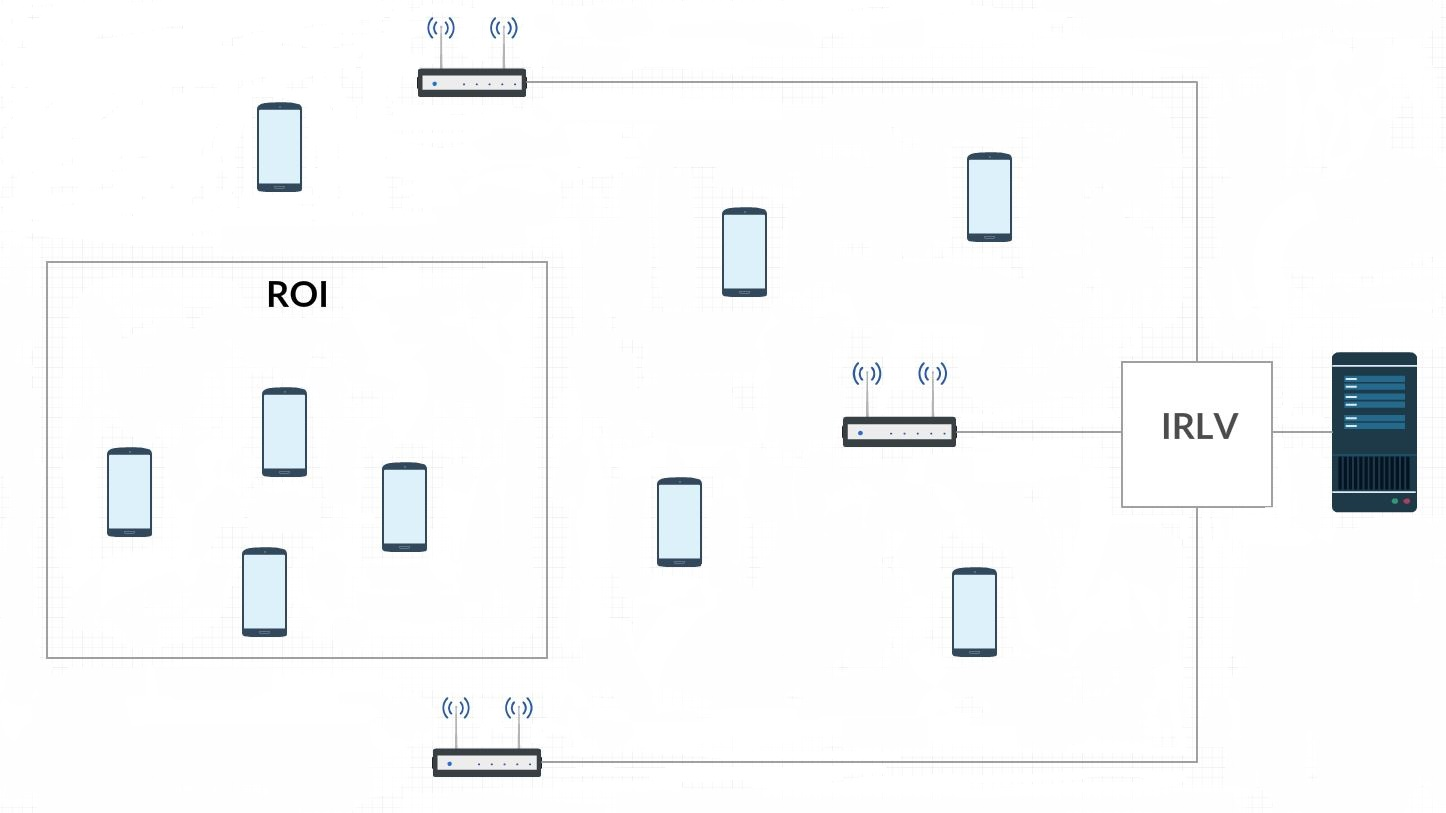
\includegraphics[width=0.6\columnwidth]{irlv.JPG}
    \caption{The considered \ac{irlv} scenario.}
    \label{fig1}
\end{figure}

With reference to Fig. \ref{fig1} We consider a cellular system with $N_{\rm AP}$ \acp{ap} covering the area $\mathcal{A}$ over a plane. We propose a \ac{irlv} system to determine if a \ac{ue} is transmitting from within an {\em authorized} \ac{roi} $\mathcal{A}_0$ within   $\mathcal{A}$. The complementary region to the \ac{roi} is  $\mathcal{A}_1=\mathcal{A} \setminus \mathcal{A}_0$. The authentication process exploits the location dependency of the features of the channel between the \ac{ue} and the \acp{ap}.  Among the various features (e.g., power, impulse response, phase offset) for the sake of a simpler exposition we consider a narrowband transmission and we focus on the power attenuation along the channel between the  \acp{ap} and the \ac{ue}. Extensions of the technique to more elaborate channel features is straightforward and its evaluation is left for future study.

The exploitation of the channel features is obtained by letting the \ac{ue} transmit a training signal, known at the \acp{ap}, from which the \acp{ap} can estimate the received power, from which a measure of the attenuation incurred along the channel is obtained. We assume that the attenuation estimation is perfect, thus not affected by noise or interference: this can be achieved by using a long enough training signal.




\subsection{Channel Model}


When the \ac{ue} transmits with power $P_{\rm tx}$, the received power at the $n^{\rm th}$ \ac{ap} is
\begin{equation}\label{eq: rec pow}
    P_{\rm rc}^{(n)}= \frac{P_{\rm tx}}{a^{(n)}},
\end{equation}
where $a^{(n)}$ is the attenuation incurred over the channel between the \ac{ue} and the \ac{ap} $n$. The channel model for path loss and shadowing is derived from \cite{3gpp}. The attenuation coefficient includes the effects of path-loss, shadowing and fading. In particular, assuming Rayleigh fading we have 
\begin{equation}
    \sqrt{a^{(n)}} \sim \mathcal{N}\left(0,\sigma_{a,n}^2\right),
\end{equation}
where $\sigma_{a,n}^2={P_{\ell}^{(n)}}e^{s}$ accounts for the path loss and shadowing components, as $P_{\ell}^{(n)}$ is the path-loss coefficient and $s \sim \mathcal{N}(0,\sigma_s^2)$ is the shadowing component.

The  path loss and shadowing modes are  derived from \cite{3gpp}. In particular, let us denote as $\bm{x}_{\rm bs}^{(n)} =(X_{\rm bs}^{(n)},Y_{\rm bs}^{(n)})$ the position of  \ac{ap} $n= 1, \ldots, N_{\rm AP}$. For a \ac{ue} located at $\bm{x}_{\rm ue}=(X_u,Y_u)$, its distance from \ac{ap} $n$ is $L(\bm{x}_{\rm ue},\bm{x}_{\rm bs}^{(n)}) = \sqrt{(X_{\rm bs}^{(n)}-X_u)^2+(Y_{\rm bs}^{(n)}-Y_u)^2}$. For the path-loss we consider two scenarios: \ac{los} and non-\ac{los}. For a \ac{los} link the path loss in dB is modelled as
\begin{equation}\label{eq:los}
    P_{\ell,{\rm LOS}}^{(n)} = 10 \nu \log_{10}\left(\frac{f 4\pi L(\bm{x}_{\rm ue},\bm{x}_{\rm bs}^{(n)})}{c}\right),
\end{equation}
where $\nu$ is the path loss coefficient, $f$ is the carrier frequency and $c$ is the speed of light. 
For a  non-\ac{los} link the path loss coefficient in dB is defined as
\begin{equation}
    P_{\ell, {\rm NLOS}}^{(n)} = 40\log_{10}\left (\frac{L(\bm{x}_{\rm ue},\bm{x}_{\rm bs}^{(n)})}{10^3}\right ) + 21\log_{10}\left(\frac{f}{10^6}\right) + 80.
\end{equation}

The shadowing parameter $s$ is zero-mean Gaussian distributed with power $\sigma^2_s$. Moreover, the shadowing parameters of two \acp{ue} located at positions $\bm{x}_i$ $\bm{x}_j$ and transmitting to the same \ac{ap} are correlated Gaussian variables with correlation $\sigma_s^2e^{-\frac{L(\bm{x}_i,\bm{x}_j)}{d_c}}$, where $d_c$ is the shadowing decorrelation distance. 

Path-loss and shadowing are assumed to be time-invariant, while the fading component is independent at each attenuation estimate. 

\subsection{\ac{irlv} With Known Channel Statistics}\label{sec:auth}

The \ac{irlv} problem can be seen as an hypothesis test between the two hypothesis (events):
\begin{itemize}
    \item $\mathcal{H}_0$: the \ac{ue} is transmitting from area $\mathcal{A}_0$;
    \item $\mathcal{H}_1$: the \ac{ue} is transmitting from area $\mathcal{A}_1$.
\end{itemize}
Given vector $\bm{a} = [a^{(1)}, \ldots, a^{(N_{\rm AP})}]$ collecting the attenuation estimates at all the \acp{ap}, we aim  at determining the most likely hypothesis, in order to perform  \ac{irlv}. While a few measurements of path-loss would allow by triangulation to establish the exact position of the \ac{ue}, the presence of shadowing and fading makes the \ac{irlv} more problematic and in general prone to errors. Let us indicate with $\hat{\mathcal H} \in  \{\mathcal{H}_0, \mathcal{H}_1\}$ the decision taken at the \acp{ap} on the two hypothesis, and let $\hat{\mathcal H} \in  \{\mathcal{H}_0, \mathcal{H}_1\}$ the ground true, i.e., the effective location of the \ac{ue}. We have two possible errors: \acp{fa}, which occur when the \ac{ue}  is classified as outside the \ac{roi}, while being inside it, and \acp{md}, which occur when the \ac{ue}  is classified as inside the \ac{roi}, while being outside of it. We also indicate the \ac{fa} probability  as $P_{\rm FA} =P(\hat{\mathcal H} = \mathcal H_1 | \mathcal H = \mathcal H_0)$ and the \ac{md} probability as $P_{\rm MD}=P(\hat{\mathcal H} = \mathcal H_0 | \mathcal H = \mathcal H_1)$.

Now, let  $p(\bm{a}|\mathcal{H}_i)$ be the probability of estimating the vector $\bm{a}$ given that  $\mathcal{H} = \mathcal{H}_i$. The \ac{llr} for the considered hypothesis is defined as 
\begin{equation}\label{eq:lr}
    {\mathcal M}(\bm{a})=\ln\left(\frac{p(\bm{a}|\mathcal{H}_0)}{p(\bm{a}|\mathcal{H}_1)}\right).
\end{equation}
According to the \ac{np} theorem, the most powerful test is obtained by comparing $\mathcal{M}(\bm{a})$ with a threshold value $\Lambda$, i.e., obtaining the test function
\begin{equation}
\label{eq:oneClassDec}
f^*(\bm{a}) =
\begin{cases}
1 &\text{if } {\mathcal M}(\bm{a}) \geq \Lambda \\
-1 & \text{if } {\mathcal M}(\bm{a}) < \Lambda,
\end{cases}
\end{equation}
This procedures  provides the minimum \ac{md} probability for a given  \ac{fa} probability.

\subsection{Example of \ac{np} Test}\label{sec:los}

We provide here an example of application of the \ac{np} theorem to a simplified scenario. Consider the overall network area as a circle $\mathcal{C}$ with radius $R_{\rm out}$ and assume a single \ac{ap} ($N_{\rm ap} =1$) located at the center of $\mathcal{C}$. The \ac{roi} $\mathcal{A}_{0}$ is a rectangle of height $H$ and length $L$ and with nearest point to the center of $\mathcal{C}$ at a distance $R_{\rm min}$. The channel model includes only path-loss (without shadowing and fading), in a \ac{los} scenario, therefore $a$ is given by (\ref{eq:los}). We notice that the attenuation is a deterministic function of the distance $R$, hence once an attenuation value is measured by the \ac{ap} the system computes the distance from the \ac{ap} and the \ac{ue}.
\begin{equation}
    R = \frac{c\sqrt[\leftroot{-3}\uproot{3}\nu]a}{f 4 \pi}
\end{equation}

 The probability that the \ac{ue} is located at a distance $R\le R_0$ in $\mathcal{A}_0$ is
\begin{equation}\label{eq:cdf}
     F(R_0) = \mathbb{P}(R \le R_0|\mathcal{A}_0) = \frac{1}{|\mathcal{A}_0|}\int_{R_{\rm min}}^{R_0} \rho  \zeta(\rho ) d\rho ,
\end{equation}
where $\zeta(\rho )$ denotes the angle of the circular sector located at distance $\rho$ intersecting area $\mathcal{A}_0$. By taking the derivative of (\ref{eq:cdf}) respect to $R_0$ we obtain the \ac{pdf} of $R_0$ given that the \ac{ue} is located in $\mathcal{A}_0$, i.e.,
\begin{equation}\label{eq: num}
    p_{R|\mathcal{A}_0}(R_0 |\mathcal{A}_0) = \frac{1}{|\mathcal{A}_0|}R_0 \zeta(R_0).
\end{equation}
Following the same reasoning and considering that the length of the arc of circle with radius $R_0$ located in $\mathcal{A}_1$ is $2\pi - \zeta(R_0)$, we obtain the \ac{pdf} of  $R$ given that the \ac{ue} is located in $\mathcal{A}_1$ as
\begin{equation}\label{eq: den}
     p_{R|\mathcal{A}_1}(R_0 |\mathcal{A}_1) = \frac{1}{|\mathcal{A}_1|}R_0 \left(2\pi-\zeta(R_0)\right),
\end{equation}
From (\ref{eq: num}) and (\ref{eq: den}) we obtain the \ac{llr} as a function of the \ac{ue}'s distance from the \ac{ap} as
\begin{equation}
    \mathcal{M}(R_0) = \frac{|\mathcal{A}_1|\zeta(R_0)}{|\mathcal{A}_0|\left(2\pi-\zeta(R_0)\right)}
\end{equation}

\section{\Ac{irlv} by Machine Learning Approaches}


The application of the \ac{np} theorem requires the knowledge of the conditional channel statistics $p(\bm{a}|\mathcal{H}_i)$ at the \acp{ap}, which can be hard to obtain, also because a-priori assumptions on their expressions may be quite unrealistic. 
 Therefore, we propose to use a \ac{ml} approach that requires two phases:
\begin{itemize}
    \item {\em Learning phase}: the \ac{ap} collects attenuation vectors from a trusted \ac{ue} moving both inside and outside the \ac{roi}, and the \ac{ue} reports its position to the \acp{ap}. Therefore the \acp{ap} can learn the behaviour of the attenuation in the two regions $\mathcal A_0$ and $\mathcal A_1$.
    \item {\em Exploitation phase}: the \ac{ap} verifies the location of an un-trusted \ac{ue} by the attenuation's estimate using the experience acquired in the learning phase. 
\end{itemize}

In details, the learning phase works as follows. For the attenuation vector $\ai$,  $i=1, \ldots, S$,  collected during the learning phase, there is an associated identification value $t_i$, where $t_i= -1$ if the trusted \ac{ue} is in region $\mathcal{A}_0$ and $t_i = 1$ if the trusted \ac{ue} is in region $\mathcal{A}_1$. Vector $\bm{t}=[t_1, \ldots, t_S]$ collects the labels of all the  attenuation vectors in the training phase. By these sets, the \ac{ap} design a test function  $\hat{t} = f(\bm{a})\in \{-1, 1\}$ that provides a decision for each attenuation vector $\bm{a}$. Then in the exploitation phase the \ac{irlv} algorithm computes $\hat{t} = f(\bm{a})$ for the new attenuation vectors thus taking a decision between the two hypotheses.  

Note that our solution does not explicitly evaluate the \ac{pdf} needed to compute the \ac{llr}, rather directly implement the test function.

In the rest of this Section we  briefly review the \ac{mlp} \ac{nn} and the \ac{svm}, describe the learning process  and show that in asymptotic conditions (infinite attenuation vectors in the learning phase and complex machines) the \ac{mlp} and \ac{svm} functions approximate the \ac{llr} function.
  
\subsection{Neural Networks}\label{sec:nn}

A \ac{nn} is a function of the type $\mathbb{R}^N \to \mathbb{R}^O$ which maps a set of $N$ real values into $O$ real values. A \ac{nn} processes the input in $Q$ stages, named layers, where the output of one layer is the input of the next layer. Layer $0$ with input $\bm{y}^{(0)}$ is denoted {\em input layer}, while layer $Q-1$ with output $\bm{y}^{(Q)}$ is denoted {\em output layer}, while intermediate layers are denoted {\em hidden layers}. 

Layer $\ell$ has $N^{(\ell)}$ outputs obtained by processing the inputs with $N^{(\ell-1)}$ functions named neurons. The output of the $n^{\rm th}$ neuron of the $\ell^{\rm th}$ layer is
\begin{equation}\label{eq:nonLin}
y_n^{(\ell+1)} = \psi\left( \bm{w}_n^{(\ell)}\bm{y}^{(\ell)}+b_n^{(\ell)} \right),
\end{equation}
i.e., the mapping by $\psi(\cdot)$ (the {\em activation function}) of the weighted linear combination with weights $\bm{w}_n^{(\ell)}$ of the outputs $\bm{y}^{(\ell)}$ of the previous layer plus a bias $b_n^{(\ell)}$. We focus here on feedforward \acp{nn}, i.e., without loops between neurons' input and output, an architecture  also known as \ac{mlp}. For a in-depth description of \acp{nn} refer for example to \cite{goodfellow}.

Various options are available in the literature for the activation functions \cite{goodfellow}. While the activation functions are typically fixed, the vectors $\bm{w}_n^{(\ell)}$ must be properly chosen to perform the desired hypothesis testing. 

In our setting, the input to the \ac{nn} is the attenuation vector $\bm{a}$ and the output layer has a unique neuron providing as output the scalar $y^{(Q)}_1$. Let $\tilde{t}(\bm{a}^{(1)})$ the output of the \ac{nn} corresponding to the attenuation vector input $\bm{a}$. The test function performs a threshold of $y^{(Q-1)}$, i.e.,
\begin{equation}
\label{testfunNN}
    f(\bm{a}) = \begin{cases}
    1 & \tilde{t}(\bm{a}) > \lambda \\
    -1 & \tilde{t}(\bm{a}) \leq \lambda.
    \end{cases}
\end{equation}
Different values of $\lambda$ provide different values of \ac{fa} and \ac{md} probabilities for this \ac{irlv} test.
   


\subsection{\ac{nn} MSE Design}
\label{sec: mse_train}

During the learning phase the \ac{mlp} parameters are designed in order to minimize 
the \ac{mse} 
\begin{equation}
\Gamma = \sum_{i=1}^S |\tilde{t}(\ai) - t_i|^2.
\end{equation}
This is achieved by using the stochastic gradient descent algorithm \cite{Bishop2006}.

We now prove the connection of \ac{mse} training with the \ac{np} theorem.
\begin{theorem}
\label{th:nn_np}
Consider a \ac{mlp} with perfect training and a sufficient number of parameters such that training reaches a global minimum. Then the hypothesis test obtained by minimizing the \ac{mse} in the learning phase is equivalent to the hypothesis test obtained via \ac{np} lemma.
\end{theorem}
\begin{proof}
It has been shown in \cite{Ruck-90} that a \ac{mlp} trained via \ac{mse} implements a function that is the minimum \ac{mse} approximation of the Bayes optimal discriminant function
\begin{equation}\label{eq:bayesDisc}
g_0(\bm{a}) = \mathbb{P}(\mathcal{H}=\mathcal{H}_0|\bm{a}) - \mathbb{P}(\mathcal{H}=\mathcal{H}_1|\bm{a}).
\end{equation} 
By recalling that $\mathbb{P}(A|B)=\mathbb{P}(B|A)\mathbb{P}(A)/\mathbb{P}(B)$ for any events $A$ and $B$, we can write
\begin{equation}
g_0(\bm{a}) = \frac{p(\bm{a}|\mathcal H_0){\mathbb P}(\mathcal{H}=\mathcal H_0) - p(\bm{a}|\mathcal H_1){\mathbb P}(\mathcal{H}=\mathcal H_1)}{\mathbb p(\bm{a})},
\end{equation}
which in turn can be written as
\begin{equation}
g_0(\bm{a}) = \frac{p(\bm{a}|\mathcal H_0){\mathbb P}(\mathcal{H}=\mathcal H_0) - p(\bm{a}|\mathcal H_1){\mathbb P}(\mathcal{H}=\mathcal H_1)}{p(\bm{a}|\mathcal H_0){\mathbb P}(\mathcal{H}=\mathcal H_0) + p(\bm{a}|\mathcal H_1){\mathbb P}(\mathcal{H}=\mathcal H_1)}.
\end{equation}
By imposing a threshold $\lambda$ on $g_0(\bm{a})$ and reorganizing we obtain
\begin{equation}
\frac{p(\bm{a}|\mathcal H_0)}{p(\bm{a}|\mathcal H_1)}> \frac{1 + \lambda}{1-\lambda} \, \frac{{\mathbb P}(\mathcal{H}=\mathcal H_1)}{{\mathbb P}(\mathcal{H}=\mathcal H_0)}  = \lambda^*,
\end{equation}
which is equivalent to the \ac{np} criterion.
\end{proof}

\subsection{\ac{nn} CE Design}
\label{sec: ce_train}
 
In this case the \ac{mlp} parameters are chosen in order to minimize the \ac{ce}  
\begin{equation}\label{eq:ce}
\chi = -\sum_{i=1}^{S} t_i\ln(\tilde{t}(\ai))+(1-t_i)\ln( 1-\tilde{t}(\ai).
\end{equation}
 
When training is performed with \ac{ce} loss function the output of the \ac{mlp} is the minimum \ac{mse} approximation of the probability $\mathbb{P}(\mathcal{H}_0|\bm{a}^{(i)})$ of being in hypothesis $\mathcal{H}_0$ given that the attenuation vector is $\bm{a}$ \cite{Bishop2006}, i.e.,
\begin{equation}
    \tilde{t}(\bm{a}) \approx \mathbb{P}(\mathcal{H}=\mathcal{H}_0|\bm{a})\,,
\end{equation} 
where the approximation is in the \ac{mse} sense.

We then have the following result
\begin{theorem}
\label{th:nn_np2}
Consider a \ac{mlp} with perfect training and a sufficient number of parameters such that the training reaches a global minimum. Then the classifier obtained by training the \ac{mlp} via \ac{ce} is equivalent to the classifier obtained via \ac{np} lemma.
\end{theorem}
\begin{proof}
Since we are considering a two-class classification problem the probability $\mathbb{P}(\mathcal{H} =\mathcal{H}_1|\bm{a}^{(i)})$, i.e., the probability of being in hypothesis $\mathcal{H}_1$ given that the attenuation vector is $\bm{a}$, is obtained as
\begin{equation}
    \mathbb{P}(\mathcal{H} = \mathcal{H}_1|\bm{a} ) = 1- \mathbb{P}(\mathcal{H} = \mathcal{H}_0|\bm{a} ).
\end{equation}
By imposing a threshold on the output of the \ac{nn} we obtain
\begin{equation}
    \mathbb{P}(\mathcal{H}=\mathcal{H}_0|\bm{a}) \approx  f(\bm{a}) \gtrsim \lambda,
\end{equation}
which can be rewritten as
\begin{equation}
    2\mathbb{P}(\mathcal{H}=\mathcal{H}_0|\bm{a} )-1 \gtrsim \hat{\lambda}
\end{equation}
\begin{equation}
    \mathbb{P}(\mathcal{H}=\mathcal{H}_0|\bm{a} )-(1-\mathbb{P}(\mathcal{H}=\mathcal{H}_0|\bm{a} )) \gtrsim \hat{\lambda}
\end{equation}
\begin{equation}
\label{lasteq}
    \mathbb{P}(\mathcal{H}=\mathcal{H}_0|\bm{a} )-\mathbb{P}(\mathcal{H}=\mathcal{H}_1|\bm{a} ) \gtrsim \hat{\lambda}.
\end{equation}
We thresholding the output of the \ac{nn} trained with the \ac{ce} criterion is equivalent to performing (\ref{lasteq}), which in turn coincides (apart for a different threshold name) with the function performed by the \ac{nn} trained with the \ac{mse} criterion, as shown in (\ref{eq:bayesDisc}). Therefore, from Theorem 1 we conclude that also the \ac{ce} training provides a test function equivalent the \ac{np} test function.
\end{proof}

\subsection{Support Vector Machine}\label{sec:svm}
A \ac{svm} \cite{Bishop2006} is a supervised learning model that can be used for classification and regression. We focus here on binary classification to solve the \ac{irlv} problem. The \ac{svm} solution comprises the function $\tilde{t}(\bm{a}): \mathbb{R}^{N_{\rm AP}} \to \mathbb{R}$ defined by
\begin{equation}
\label{eq:svm}
\tilde{t}(\bm{a}) = \bm{w}^T \phi (\bm{a}) + b,
\end{equation}
where $\phi: \mathbb{R}^{N_{\rm AP}} \to \mathbb{R}^K$ is a feature-space transformation function, $\bm{w} \in \mathbb{R}^K$ is the weight vector and $b$ is a bias parameter, and the test function is again provided by (\ref{testfunNN}) where now $\tilde{t}(\bm{a})$ is given by (\ref{eq:svm}). Note that in the classical \ac{svm} formulation we have $\lambda = 0$.

While the feature-space transformation function is typically fixed,  vector $\bm{w}$ must be properly chosen to perform the desired hypothesis testing. 

\subsection{\ac{svm} LS Design}

For the the choice of the \ac{svm} parameters we consider the \ac{lssvm} approach \cite{Suykens1999}.  Learning for \ac{lssvm} is performed by solving the following optimization problem
\begin{subequations}
	\label{eq:lssvm}
	\begin{equation}
	\label{eq:lssvmOrig}
	\underset{\bm{w},b }{\text{min}} \quad \omega(\bm{w},b) \triangleq \frac{1}{2} \bm{w}^T \bm{w} + C \frac{1}{2} \sum_{i=1}^S e_i ^2 
	\end{equation}
	\begin{equation}
	\label{eq:stpart}
	e_i =   t_i[\bm{w}^T \phi (\bm{a}^{(i)}) + b]-1   \quad i = 1 ,\dots,S\,,
	\end{equation}
\end{subequations}
where $C$ is a hyper-parameter. In the traditional \ac{svm}, variables $e_i$ are constrained to be non-negative and appear in the objective function as is. Inequalities in the constraints translates into a quadratic programming problem, while equalities constraints in \ac{lssvm} yield a linear system of equations in the optimization values. In \cite{Yevs} it is shown that \ac{svm} and \ac{lssvm} are equivalent under mild conditions.

From the constraints in \eqref{eq:lssvm} and the fact that $t_i = \pm 1$ we have
\begin{equation}
\label{eq:els}
e_i^2 = (1 - t_i\tilde{t}(\bm{a}^{(i)}) )^2 = (t_i - \tilde{t}(\bm{a}^{(i)}))^2,
\end{equation}
that is the squared error between the soft output of the \ac{lssvm} $\tilde{t}(\bm{a}^i)$ and the correct training label $t_i$.

We now prove the equivalence between the \ac{lssvm} and \ac{np} classifiers. Let us first consider the following lemma that establishes the convergence of the learning phase of \ac{svm}, as the training sample set becomes large.

\begin{lemma}
	\label{lem:lem1}
	For large number of training samples $\bm{a}^{(i)}$ taken with a given static probability distribution from a finite alphabet $\mathcal C$, i.e., for$S \rightarrow \infty$, the vector $\bm{w}$ of the \ac{lssvm} converges in probability to a vector of finite norm $||\bm{w}||_2 = \bm{w}^T\bm{w}$.
\end{lemma}

\begin{proof}
See the Appendix.
\end{proof}
 
We are now ready to proof the the following theorem establishing the optimality of the \ac{svm} solution, as it provides the most powerful \ac{np} test, for a given \ac{fa} probability.

\begin{theorem}
	\label{th:lsnp}
	Consider a \ac{lssvm} with perfect training, \ie the training reaches a global minimum of $\omega(\bm{w},b)$ given an infinite number of training points $\bm{a}^{(i)}$ drawn from the finite alphabet $\mathcal C$. Then the test function obtained by training the \ac{lssvm} and by thresholding the soft output \eqref{eq:svm} is equivalent, in the \ac{mse} sense, to the \ac{np} test function.
\end{theorem}
\begin{proof}
	From \eqref{eq:lssvmOrig} consider
	\begin{equation}
	\label{eq:lssvmDim1}
	\lim_{S \to +\infty} \frac{1}{S} \omega(\bm{w},b) =\frac{C}{2} \lim_{S \to +\infty}\frac{1}{S}  \sum_{i=1}^S e^2_i	=\frac{C}{2}\E_t(\bm{w},b),
	\end{equation}
	where $\E_t(\bm{w},b) = \Exp{\left(t_i - \tilde{t}(\bm{a}^{(i)})\right)^2} $ is the expected value carried out \wrt the training points $\bm{a}^{(i)}$, as $S$ goes to infinity. 	The first equality in\eqref{eq:lssvmDim1} comes from Lemma 1: since $\bm{w}$ converges to a finite norm, we can write
	\begin{equation}
	\lim_{S\to \infty} \frac{1}{S} \bm{w} \bm{w}^T 	= 0.
	\end{equation} 
	The last equality comes from the strong law of large numbers. In the limit, the optimization problem \eqref{eq:lssvm} is equivalent to
	\begin{equation}
	\label{eq:lsInf}
	\begin{aligned}
	& \underset{\bm{w},b}{\text{min}} & &  \E_t(\bm{w},b), & 
	\end{aligned}	
	\end{equation}
	where we dropped the constraints in \eqref{eq:lssvm} by substitution using \eqref{eq:els}. The optimization problem is the same as in the \ac{nn} case and from \cite{Ruck-90} we have that the couple $(\bm{w}^*,b^*)$ minimizing \eqref{eq:lsInf} and parametrizing \eqref{eq:svm} is such that with these parameters of the \ac{svm}
	\begin{equation}
	\tilde{t}(\bm{a}^i)  \approx \mathbb{P}(\mathcal{H}_0|\bm{a}^{(i)}) - \mathbb{P}(\mathcal{H}_1|\bm{a}^{(i)}).
	\end{equation}
	Lastly, we exploit Theorem \ref{th:nn_np} to conclude the \ac{np}-optimality of the \ac{ls}-\ac{svm}.
\end{proof}

%It is common practice in the literature \cite{Bishop2006,Suykens1999} to work with the dual formulation of the optimization problems \eqref{eq:svmS} to \eqref{eq:lssvm} by constructing the Lagrangian. 
%In the dual formulation objective functions and constraints are expressed as functions of the kernel 
%\begin{equation}
%	\psi(\bm{r}_i,\bm{r}_j) = \phi (\bm{r}_i)^T \phi(\bm{r}_j),	
%\end{equation}
%without explicitly defining the function $\phi(\cdot)$. 
%The output of $\phi(\cdot)$ can now be of infinite dimension, like with the radial kernel family
%\begin{equation}
%	\psi(\bm{r}_i,\bm{r}_j; \sigma) = \exp \left( \frac{|| \bm{r}_i - \bm{r}_j ||^2}{2\sigma^2} \right).
%\end{equation}
%In this case, Theorem \ref{th:lsnp} holds only if
%\begin{equation}
%	\lim_{S \to +\infty} \frac{1}{S} \bm{w}^T \bm{w} < +\infty.	
%\end{equation} 
%However, if we let $C \to +\infty$ in \eqref{eq:lssvm}

\section{\ac{irlv} By One-class Classification}
\label{sec:OneClass}
 

In practice having learning points in both regions $\A{0}$ and $\A{1}$ may be difficult since $a$) region $\A{1}$ may be quite wide and not necessarily well defined (being simply the complementary region of $\A{0}$) and $b$) the attacker may use multiple antennas and by beamforming  can induce attenuation estimates that not necessarily correspond to points in the region $\A{1}$. %About point b), we will further discuss attack possibilities in Section \ref{sec:attack}.

Due to inconsistencies of attenuation vectors not belonging to region $\A{0}$, we propose here an \ac{irlv} system that during the identification association (or learning) phase uses only samples obtained from region $\A{0}$. This problem can also be denoted as one-class classification since we know only samples taken from one of the classes of the classifier. 

We now discuss the one-class classification problem implemented via both \ac{nn} and \ac{svm}.
 

\subsection{Test Function With Known Statistics}
\label{sec:oneClassOpt}

In the one-class scenario the \ac{llr} \eqref{eq:lr} can not be used as discriminant function, as $p(\bm{a}|\mathcal{H}_1)$ is not known. In this case we can resort to the \ac{glrt} \cite{Kay-book}, which, although not proven to be optimal, is a meaningful generalization of the \ac{np} test. Hence the test function becomes 
%
%Consider the probability of classification error
%\begin{equation}
%    p_e = {\mathbb P}\left(\hat{\mathcal H} = \mathcal{H}_0|{\mathcal H} = \mathcal{H}_1 \right){\mathbb P}\left({\mathcal H}=  \mathcal{H}_1\right)+{\mathbb P}\left(\hat{\mathcal H} = \mathcal{H}_1|{\mathcal H} = \mathcal{H}_0 \right){\mathbb P}\left( {\mathcal H} = \mathcal{H}_0\right)
%\end{equation}
%that can be rewritten as
%\begin{equation}
%   p_e = \int p_e(\bm{a}) d\bm{a}, 
%\end{equation}
%where 
%\begin{equation}\label{eq: disc}
%    p_e(\bm{a}) = {\mathbb P}\left( \hat{\mathcal H} = \mathcal{H}_0|\mathcal{H}=\mathcal{H}_1\right)p\left(\bm{a}|\mathcal{H}_1\right)+{\mathbb P}\left(\hat{\mathcal H} = \mathcal{H}_1|\mathcal{H}= \mathcal{H}_0\right){\mathbb P}\left(\bm{a}|\mathcal{H}_0\right)
%\end{equation}
%is the error \ac{pdf} for a given attenuation vector $\bm{a}$.
%
%\colorbox{yellow}{qui non capisco}
%In order to minimize $p_e(\bm{a})$ we can then consider the following test function
%\begin{equation}
%f(\bm{a})=    \begin{cases}
%    1 & \text{if }   p\left(\bm{a}|\mathcal{H}_0\right)  \geq \lambda \\
%-1 & \text{if }
%  p\left(\bm{a}|\mathcal{H}_0\right) < \lambda\,,
%    \end{cases}
%\end{equation}
%
%However, since we do not know the statistics of the attenuation vectors in hypothesis $\mathcal{H}_1$ and the prior probabilities of both hypothesis, we move all the unknown terms to the right side of the inequality, obtaining  
\begin{equation}
\label{eq:oneClassDec}
f^*(\bm{a}) =
\begin{cases}
1 &\text{if } p(\bm{a}|\mathcal{H}_0) \geq \Lambda \\
-1 & \text{if } p(\bm{a}|\mathcal{H}_0) < \Lambda,
\end{cases}
\end{equation}
which represents the best discriminant function for the one-class classification problem.


\subsection{Auto Encoder \ac{nn}}
\label{sec:auto}

When attenuation statistics conditioned to the two hypothesis are not available, we can apply \ac{ml} solutions, as for the case of two-classes classification of Section III. 

In particular we consider here the \ac{ae} \cite{Hinton-2006}, i.e., a \ac{nn} that is trained to: $a$) convert high-dimensional inputs to low-dimensional vectors in the hidden layer; $b$) reconstruct the high-dimensional input at the output layer from the low-dimensional vectors of the hidden layer. Therefore the size of the hidden layer is smaller than the size of the input layer, i.e., when $M<N$ \cite{Bourlard-88}. The capacity of the auto-encoder to replicate only certain values at the output is due to the fact that the hidden layer is able the extract the features of the training set. The simplest architecture for \ac{ae} is a feedforward \ac{nn} with three layers, i.e., a size $N$ input layer, a size $M$ hidden layer and a size $N$ output layer, as shown in figure \ref{fig:aeArch}. In this case it is convenient to use a linear activation function when mapping the hidden layer to the output layer \cite{goodfellow}. Note that the output of the \ac{ae} is a vector of the same size of the \ac{ae} input. The \ac{ae} can be used to perform one-class classification by computing the reconstruction error between the input and the output of the \ac{ae} and comparing its absolute value with a chosen threshold.

\begin{figure}[t]
    \centering
    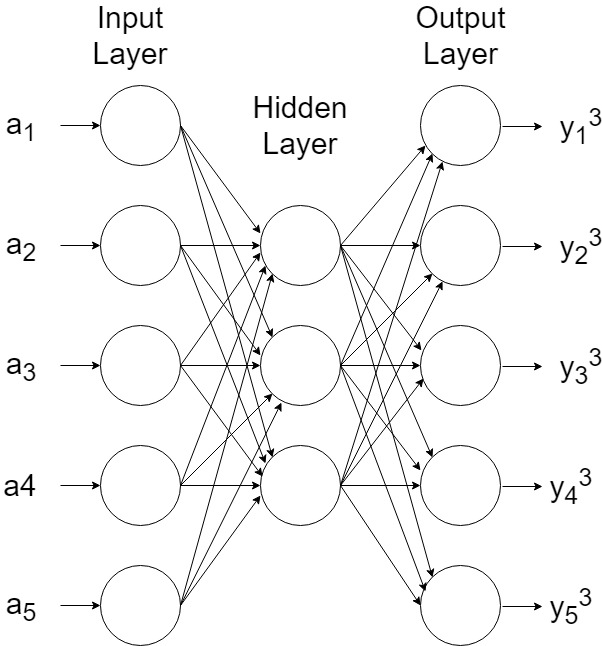
\includegraphics[width=0.5\columnwidth]{AE.jpg}
    \caption{Example of \ac{ae} architecture with $5$ input (and output) values and one hidden layer with 3 neurons.} 
    \label{fig:aeArch}
\end{figure}

For our \ac{irlv} problem, we train the \ac{ae} with attenuation vectors $\bm{a}^{(i)}$ taken only when the trusted \ac{ue} is in the \ac{roi} $\mathcal A_0$. Then, by letting $\bm{y}^{(L)}$ be the output of the \ac{ae} for the attenuation input $\bm{a}$, the reconstruction error is 
\begin{equation}\label{eq: rec err}
    \epsilon(\bm{a} ) = \frac{1}{N}\sum_{n=1}^{N}|a_n-y^{(L)}_n|^2.
\end{equation}
Finally, the \ac{irlv} test function  is  
\begin{equation}
f(\bm{a}) =
\begin{cases}
1 &\text{if } \epsilon(\bm{a} ) \geq \Lambda \\
-1 & \text{if } \epsilon(\bm{a} ) < \Lambda,
\end{cases}
\end{equation}

About the test power of the \ac{ae}, we observe that it can be seen as a quantization (or compression process) that quantizes an $N$-dimensional signal into an $M$-dimensional signal. In order to minimize the \ac{mse} of the reconstruction error, inputs with higher probability will have smaller quantization regions. Moreover, as the number of quantization points goes to infinity (since the quantization indices are in the continuous $M$-dimensional space) all points in the same quantization region will have approximately the same probability. However, quantization error for points within each region will be different for each points, in particular being zero for the quantization point and higher at the edges of the quantization region. Thus we can conclude that even with infinite training and an infinite number of neurons the \ac{ae} can not provide as output the \ac{pdf} of the input, as required by the optimal decision rule (\ref{eq:oneClassDec}). On the other hand, input points with a smaller \ac{pdf} belong to larger quantization regions for which the reconstruction error is {\em on average} larger, thus on average the output provided by the autoencoder is monotonically decreasing with the \ac{pdf} of the input point. 

\begin{comment}
The performance of the obtained classifier are given by the following 
\begin{theorem}
    Consider a \ac{ae} with perfect training, i.e., a \ac{ae} with a sufficient number of neurons and a sufficient training. Then the classifier obtained by training the \ac{ae} and by thresholding the soft output $\tilde{\epsilon}(\bm{a}^{(n)}) = \sqrt{\frac{1}{N}\sum_{i=1}^{N}|a^{(n)}_i-\hat{a}^{(n)}_i|^2},$ is equivalent, in the \ac{mse} sense, to the optimal classifier \eqref{eq:oneClassDec}.
\end{theorem}
\begin{proof}
Let us consider the \ac{mse} approximation of $\tilde{\epsilon}(\bm{a}^{(n)})$ being $1/p(\bm{a}^{(n)}|\mathcal{H}_0)$ and hence consider the minimization problem over the weight vector $\bm{w}$
\begin{equation}
	\begin{aligned}
		&\underset{\bm{w}}{\text{min}}\,\, \Exp{ \left( \tilde{\epsilon}(\bm{a},\bm{w}) - \frac{1}{p(\bm{a}|\mathcal{H}_0)}\right) ^2} = \\
		&\underset{\bm{w}}{\text{min}} \int_{\bm{a} \in \mathbb{R}^n} \left[ \tilde{\epsilon}(\bm{a},\bm{w}) - \frac{1}{p(\bm{a}|\mathcal{H}_0)} \right] ^2 p(\bm{a}|\mathcal{H}_0) d\bm{a} = \\
		&\underset{\bm{w}}{\text{min}} \left\lbrace \int_{\bm{a} \in \mathbb{R}^n} \tilde{\epsilon}(\bm{a},\bm{w})^2 p(\bm{a}|\mathcal{H}_0) d\bm{a}
		-2\int_{\bm{a} \in \mathbb{R}^n} \tilde{\epsilon}(\bm{a},\bm{w}) d\bm{a}
		+ \int_{\bm{a} \in \mathbb{R}^n} \frac{1}{p(\bm{a}|\mathcal{H}_0)} d\bm{a} \right\rbrace.
	\end{aligned}	
\end{equation}
We notice that the second term in brackets is the sum of the reconstruction error of the attenuation vectors over $\mathbb{R}^{n}$. Since different regions of $\mathbb{R}^n$ are characterized by different features and since the \ac{ae} is able to reconstruct, with small reconstruction error, only those vectors with features similar to those of the training set we can assume that the summation of the reconstruction errors over all possible feature spaces goes to infinity. The second integral does not hence depend on $\bm{w}$ as for each value of $\bm{w}$ it goes to infinity. The last term in brackets does not depend on the weight vector $\bm{w}$ and hence the only term that depends on $\bm{w}$ is the first one, which is the objective function of the training optimization problem. Noticing that thresholding $\frac{1}{p(\bm{a}|\mathcal{H}_0)}$ with $\gamma$ is equivalent to thresholding $p(\bm{a}|\mathcal{H}_0)$ with $1/\gamma$ we conclude that training the \ac{ae} with $\epsilon$ loss function provides a classifier that approximates in the \ac{mse} sense the optimal one (\ref{eq:oneClassDec}).
\end{proof}
\end{comment}

\subsection{One-Class LS-SVM}

Similarly, we can resort to \ac{svm} to perform the one-class classification in \ac{irlv}. We focus in particular on the  \ac{oclssvm}, first introduced in \cite{choi2009least} as an extension of the one-class \ac{svm} \cite{Scholkopf2001estimating}. 

The only difference with respect to the \ac{svm} introduced in Section III is that the training optimization problem is now
\begin{subequations}
	\label{eq:oneClassSvm}
	\begin{equation}
	\label{eq:oneClass1}
	\underset{\bm{w},b}{\min} \quad \phi(\bm{w}, b) \triangleq
	 \frac{1}{2} \bm{w}^T \bm{w} +  \frac{C}{2} \sum_{i=1}^S e_i^2 +b
	\end{equation}
	\begin{equation}
	\label{eq:oneClassConstr}
	\text{subject to}\, -b - \bm{w}^T \phi (\bm{a}^{(i)})  = e_i,  \quad i = 1,\dots S, 
	\end{equation}
\end{subequations}
where $C$ is a hyper-parameter.
Note that in the one-class case, the bias parameter $b$ appears also in the objective function.


Also in this case we observe that the one-class \ac{svm} is suboptimal, as it does not provides a monotone function of the \ac{pdf} of the input points. In fact, it is not necessary that each training point further away from the bound of the classification region is less probability and the direction $\bm{w}$ is obtained by an ensemble elaboration of the \ac{pdf} of the input rather then been a point-wise function of it. Still, by resorting to the Chernoff bound we can conclude that by minimizing the \ac{mse} we also minimize the upper bound the probability of false alarm, thus although not optimal, the optimization process goes in the right direction.



\begin{comment}
We want to show that the \ac{oclssvm} is a machine that asymptotically approximate, in the mean-square sense, the optimal decision rule \eqref{eq:oneClassDec}.

\begin{lemma}
\label{lem:lem2}
Given $S$ training samples $\bm{a}^{(i)}$ from a finite alphabet $\mathcal C$, taken with a given static probability distribution, for large number of training samples, i.e., as $S \rightarrow \infty$, problem \eqref{eq:oneClassSvm} is equivalent to 
\begin{equation}
		\underset{\bm{w},e_i, \rho}{\text{min}} \Exp{e_i}^2
\end{equation}
\end{lemma}
\begin{proof}
We first proceed as in the proof of Theorem \ref{th:lsnp} and re-write problem \eqref{eq:oneClassSvm} as
	\begin{subequations}
		\label{eq:oclssvm22}
		\begin{equation}
		\label{eq:oclssvm2}
		\underset{\bm{w},e}{\text{min}} \quad f_0' = \frac{1}{2} \bm{w}^T \bm{w} + C S \frac{1}{2} \sum_{j=1}^M p_{\bm{a}^{(i)},t_i}(\bm{\alpha}_j,1) e_j^2 - \rho  
		\end{equation}
		\begin{equation}
		\label{eq:ocstpart2}
		\text{subject to}\,  \rho - \bm{w}^T \phi (\bm{a}^{(i)})  = e_i,  \quad i = 1,\dots M, 
		\end{equation}		
	\end{subequations} 
Note that differently from \eqref{eq:lssvm22} we have only $M$ constraints (and not $2M$) because we have target labels only of one class.
We now solve \eqref{eq:oclssvm22} using the same steps as in \cite{choi2009least}. Let us define the Lagrangian
\begin{equation}
	\mathcal{L} = 	\frac{1}{2} \bm{w}^T \bm{w} - \rho +
	C S \frac{1}{2} \sum_{j=1}^M p_{\bm{a}^{(i)},\hat{t}_i}(\bm{\alpha}_j,1) e_j^2 - 
	\sum_{j=1}^{M} u_j \left[ \bm{w}^T \phi (\bm{a}^{(j)}) -\rho + e_j \right],
\end{equation}
and set to zero the derivatives w.r.t. optimization variables and multipliers $u_j$

\begin{subequations}
\begin{equation}
\label{eq:derivatives1}
\frac{\partial \mathcal{L}}{\partial \bm{w}}: \quad \bm{w} = \sum_{j=1}^{M} u_j \phi (\bm{a}^{(j)}), 		
\end{equation}
  \begin{equation}
  \label{eq:derivatives2}
  		\frac{\partial \mathcal{L}}{\partial \bm{e_j}}: \quad CS p_{\bm{a}^{(i)},\hat{t}_i}(\bm{\alpha}_j,1) e_j = u_j \quad
  		 j=1,\dots, M,
  \end{equation}
  \begin{equation}
  \label{eq:derivatives3}
  		\frac{\partial \mathcal{L}}{\partial \rho}: \quad \sum_{j=1}^{M} u_j = 1
  \end{equation}
  \begin{equation}
  \label{eq:derivatives4}
  	\frac{\partial \mathcal{L}}{\partial \bm{u_j}}:	\quad \phi (\bm{a}^{(j)}) \bm{w} + e_j - \rho = 0.
  \end{equation}
\end{subequations}
Substituting \eqref{eq:derivatives1} and \eqref{eq:derivatives2} in \eqref{eq:derivatives4} we get the system of equations
\begin{equation}
\begin{aligned}
	&\sum_{i=1}^{M}  u_i k( \bm{a}^{(i)},\bm{a}^{(j)}) - \rho + \frac{u_j}{SCp_{\bm{a}^{(i)},\hat{t}_i}(\bm{\alpha}_j,1)}=0 \quad j = 1,\dots, M\\
	&\sum_{i=1}^{M}u_i=1,
\end{aligned}	
\end{equation}
with $M+1$ unknowns and $M+1$ equations which therefore provides finite convergence values for $\{\rho,u_i\}_{i=1}^{i=M}$.
In the dual formulation of \eqref{eq:oneClassSvm} we can express $\bm{w}$ as a function of the kernel and Lagrange multipliers $\{u_j\}$ 
\begin{equation}
\bm{w}^T\bm{w} = \sum_{i=1}^{M} \sum_{j=1}^{M} u_i u_j k(\bm{\alpha}_i,\bm{\alpha}_j), 
\end{equation}
which, given the finiteness of the sum, converges.
We can now write
\begin{equation}
\begin{aligned}
\lim_{S \to +\infty} &\frac{1}{S} \bm{w}^T\bm{w} =0, \\
\lim_{S \to +\infty} &\frac{1}{S}\rho =0.
\end{aligned}		
\end{equation}
It follows that
\begin{equation}
	\underset{\bm{w},e_i, \rho}{\text{min}} \frac{1}{S} f_o(\bm{w},e_i, b) = 
	\underset{\bm{w},e_i, \rho}{\text{min}} \frac{1}{S} \sum_{i=1}^S e_i^2 = 
	\underset{\bm{w},e_i, \rho}{\text{min}} \Exp{e_i}^2,	
\end{equation}
where $e_i^2 = (\bm{w}^T \phi (\bm{a}^{(i)}) -\rho)^2 $, the last equality follows from the law of large numbers, and the expected value is carried out \wrt the training $\bm{a}^{(i)}$.
\end{proof}

%Note that $|e_i|$ is proportional, by a factor $1/||\bm{w}||$, to the distance between any point $\phi(\bm{a}^{(i)})$ and the hyperplane $\bm{w}^T \phi (\bm{a}) + b = 0$ defined in the transformed space by the \ac{oclssvm}. We claim that $|e_i|$ is inversely proportional to $p(\bm{a}|\mathcal{H}_0)$ and we will prove that this holds in the mean-square sense. A direct consequence is that the \ac{oclssvm} approximates asymptotically the optimal decision rule of Section \ref{sec:oneClassOpt}. 

\begin{theorem}
	\label{th:onelsnp}
	Consider a \ac{oclssvm} with perfect training, \ie the training reaches a global minimum of $f_o(\bm{w},e_i,b)$ given an infinite number of training points $\bm{a}^{(i)}$ drawn from the finite alphabet $\mathcal C$. Then the classifier obtained by training the \ac{oclssvm} and by thresholding the soft output \eqref{eq:svm} is equivalent, in the \ac{mse} sense, to the optimal classifier \eqref{eq:oneClassDec}.
\end{theorem}

\begin{proof}
Let $(\bm{w}^*,e_i^*, \rho^*)$ be the solution for problem \eqref{eq:oneClassSvm}. We note that $\rho^* >0$. If this was not the case, then we cold define the new triplet $(-\bm{w}^*,e_i^*, -\rho^*)$ providing a lower value for $f_o(\bm{w},e_i,\rho)$. This is because from \eqref{eq:oneClass1} the first two terms of the sum remain unchanged, while in the third term we are now subtracting a positive value, yielding
\begin{equation}
		f_o(-\bm{w}^*,e_i^*, -\rho^*) < f_o(\bm{w}^*,e_i^*, \rho^*).
\end{equation} 
Let us define the function 
\begin{equation}
	e(\bm{a},\bm{w},\rho) \triangleq \bm{w}^T  \phi (\bm{a}) - \rho,	
\end{equation}
and consider 
\begin{equation}
\label{eq:coreTheorem}
	\begin{aligned}
		&\underset{\bm{w},\rho}{\text{min}} \Exp{ \left( e(\bm{a},\bm{w},\rho) - \left(-\frac{1}{p(\bm{a}|\mathcal{H}_0)}\right)\right) ^2} = \\
		&\underset{\bm{w},\rho}{\text{min}} \int_{\mathbb{R}^n} \left[ e(\bm{a},\bm{w},b) + \frac{1}{p(\bm{a}|\mathcal{H}_0)} \right] ^2 p(\bm{a}|\mathcal{H}_0) d\bm{a} = \\
		&\underset{\bm{w},\rho}{\text{min}} \left\lbrace \int_{\mathbb{R}^n} e^2(\bm{a},\bm{w},\rho) p(\bm{a}|\mathcal{H}_0) d\bm{a}
		+2\int_{\mathbb{R}^n} e(\bm{a},\bm{w},\rho) d\bm{a}
		+ \int_{\mathbb{R}^n} \frac{1}{p(\bm{a}|\mathcal{H}_0)} d\bm{a} \right\rbrace.
	\end{aligned}	
\end{equation}
Consider the integral in the double product
\begin{equation}
		\int_{\mathbb{R}^n} e(\bm{a},\bm{w},b) d\bm{a} =
		\int_{\mathbb{R}^n} \bm{w} ^T  \phi (\bm{a})d\bm{a} - \int_{\mathbb{R}^n} \rho d\bm{a},		
\end{equation}
For what concerns the second integral in the r.h.s. we can write
\begin{equation}
		\int_{\mathbb{R}^n} \rho d\bm{a} = \rho \int_{\mathbb{R}^n} d\bm{a} = \sign(\rho) (+\infty) = + \infty,
\end{equation}
since we have shown that at the optimum $\rho^*>0$. Now, using \eqref{eq:derivatives1}, we can write the first integral as
\begin{equation}
\begin{aligned}
		&\int_{\mathbb{R}^n} e(\bm{a},\bm{w},\rho) d\bm{a} = \int_{\mathbb{R}^n} \sum_{j=1}^{M} u_j k(\bm{a}^{(j)},\bm{a})d\bm{a} \\
		&= \sum_{j=1}^{M} u_j \int_{\mathbb{R}^n} k(\bm{a}^{(j)},\bm{a})d\bm{a} = \int_{\mathbb{R}^n} k(\bm{a}^{(j)},\bm{a})d\bm{a},
\end{aligned},
\end{equation}
where we used \eqref{eq:derivatives3}.
Note that the only term in the last line of \eqref{eq:coreTheorem} that depends on the optimization variables $\{\bm{w}, \rho \}$  is 
\begin{equation}
		\Exp{  e^2(\bm{a}, \bm{w}, \rho)} = \int_{\mathbb{R}^n} e^2(\bm{a},\bm{w},\rho) p(\bm{a}|\mathcal{H}_0) d\bm{a},
\end{equation}
which, from Lemma \ref{lem:lem2} is, asymptotically, the objective function optimized by the \ac{lssvm}.
%The third term inside the curly brackets does not depend on $(\bm{w},b)$. Therefore, the mean square error approximation of $1/p(\bm{a}|\mathcal{H}_0)$ is found by minimizing $\Exp{e^2(\bm{a},\bm{w},b)}$ which, by Lemma \ref{lem:lem2}, is the same function minimized by \ac{oclssvm}. Asymptotically we have, from \eqref{eq:svm},
%\begin{equation}
%\label{eq:approx}
%	\tilde{t} \approx \frac{1}{p(\bm{a}|\mathcal{H}_0)},	
%\end{equation} 
%in the mean square sense. Note that thresholding $\frac{1}{p(\bm{a}|\mathcal{H}_0)}$ with $\gamma$ is the same as thresholding $p(\bm{a}|\mathcal{H}_0)$ with $1/\gamma$ which is the optimal classifier of Section \ref{sec:oneClassOpt}.
\end{proof}
\end{comment}

\subsection{\ac{ml}-Based Attack Strategies}
\label{sec:attack}

\ac{ml} techniques can be also exploited in order to perform more effective attacks. In particular the attacker  $a$) obtains estimates of the attenuation vectors of its channel to all the \acp{ap}, and $b$) moves around in the area $\mathcal A_1$ and performs attacks. Point $a$) is possible if \acp{ap} transmit training signals to the \ac{ue}, so that it can estimate the channel characteristics. We also assume that the attacker has means to determine if its attack has been successful, e.g., by receiving the services reserved to \acp{ue} in the \ac{roi}.

%Consider a training set set large enough to cover the statistical description of the non-legitimate area $\mathcal{A}_1$. The attenuation vector with the highest reconstruction error in the \ac{ae} case or with the largest value of $\tilde{t}_o$ in the \ac{oclssvm} case can be considered at the border of the region $\mathcal{A}_1$, and hence nearer to region $\mathcal{A}_0$. In the next section we describe two attack strategies exploiting this property of the \ac{ml} algorithms: the former attack is the filter attack, which exploits the one class trained \ac{ml} algorithms to select proper attack vectors; the latter is the gradient based attack, which exploits the loss function of \ac{ml} algorithms in order to forge attenuation vectors that can be considered as authentic by the \ac{irlv} system.

%\subsection{Selective \ac{ml} Attack}


Although it possible to perform multiple attacks, the purpose of the attacker is to be successful with the minimum number of attacks in order not to let the network detect to be under a series of attacks and take countermeasures (e.g., activating additional \ac{irlv} techniques or switching off the service). Moreover, a smaller number of attacks reduces the resource consumption by the attacker and provides faster access to the services. In order to make attacks more efficient we propose that the attacker moves in the \ac{roi}-complementary area $\mathcal A_1$, measures the attenuation vectors at various position and then decides whether to attack or not, according to its previous experience of failed attack. We denote this attack as {\em selective \ac{ml} attack}. As soon as an attack is successful the procedure is stopped, therefore the experience on which the attacker can base its decision comprises only failed attacks.

In details, the attacker uses the attenuation vectors of (failed) attacks to train a one-class classifier. Then, when reaching a new position it feeds the attenuation vector to the classifier and it is classified as belonging to the same class of training, no attacks is performed since the position is deemed to be useless. Otherwise, if the attenuation vector is not recognized as belonging to the class of collected training, it is evaluated as a potential successful attack and the attacker sends the message attempting to be authenticated by the network. Upon success the procedure is stopped, while upon failure the attenuation vector is fed as additional training to the machine, so that the classifier becomes more accurate.  

%As before stated the one class classification involves training the \ac{ml} algorithms with attenuation vectors measured from one of the two available classes. We here propose an attack strategy which trains the \ac{ml} algorithms with attenuation vectors measured from the non-legitimate area $\mathcal{A}_1$. However, differently from a simple random attack, the attenuation vectors are \emph{filtered} by the attacker with a machine trained to learn the class of non successful points. The chosen attack point is then only the one yielding the worst metric as output of the filter. In this way we aim at minimizing the number of attempted attacks.

%In particular, consider an attenuation vector $\bm{a}_{\mathcal{A}_1}$ measured in area $\mathcal{A}_1$ This vector could be a possible successful attack and is hence tested. If the attack is not successful $\bm{a}_{\mathcal{A}_1}$ is used to train the \ac{ml} algorithm. 
%We generate $n_{\rm x}$ spatial coordinates located in area $\mathcal{A}_1$ and we measure the attenuation values incurred in each position. We then filter this set of vectors with the \ac{ml} algorithm and select as a possible attack the vector which is more likely to belong to class $\mathcal{A}_0$ (i.e., the one with highest reconstruction error for the \ac{ae} and with smallest $\tilde{t}_0$ for the \ac{oclssvm}). If the selected vector is not a successful attack then it is used to update the training of the \ac{ml} algorithm.

For the one-class classifier we use either the \ac{ae} or the \ac{svm}, as described in the previous section. 
%
% This process is repeated until a successful attack vector is generated. The algorithm steps are shown in Algorithm \ref{alg:filter}.
%
%\begin{algorithm}[t]
%\label{alg:filter}
%  \algsetup{linenosize=\tiny}
%  \scriptsize
%
% \KwData{ $\bm{a}_{\mathcal{A}_1}$}
% \KwResult{successful attack vector }
% 
%
% \Repeat{attack is successful}{
%        \eIf{first attack}{
%        test $\bm{a}_{\mathcal{A}_1}$\;
%        \If{attack $\neq$ successful}{
%        build and train the \ac{ml} architecture with $\bm{a}_{\mathcal{A}_1}$\;
%        }
%        }
%        {
%        build set $\bm{A}$ of randomly selected attenuation vectors from $\mathcal{A}_1$\;
%        $\bm{a}_{\mathcal{A}_1} = \underset{\bm{a} \in \bm{A}}{\max} \quad \rm{loss} \, \rm{function}$ $(\bm{A})$\;
%        \If{attack $\neq$ successful}{
%       update training with $\bm{a}_{\mathcal{A}_1}$
%       }
%      }
%      }
%    
% \caption{Selective \ac{ml} attack}
%\end{algorithm}

%Note that Point $b$) is possible by letting the attacker to be equipped with multiple antennas so that, thanks to the estimates its channel to the \acp{ap}, the attacker can beamform the training signals with different gains to the \acp{ap}, thus letting them estimate the intended attenuation values. In this setting even a static \ac{ue} can generate many attacks with different estimated attenuation vectors at the \acp{ap}. 

% \subsection{Gradient-based \ac{ae} attack}
% Consider the set $\bm{A}$ of the attenuation vectors from $\mathcal{A}_1$ used for training the attacker \ac{ae}. The vector with highest reconstruction error is selected as a starting point for a possible successful attack. In order to find a direction toward which move the values of the attenuation vector to increment the probability of a successful attack, knowing that a higher reconstruction error means an higher probability of the vector belonging to the authentic area $\mathcal{A}_0$, we perform a gradient ascent algorithm based on the reconstruction error function (\ref{eq: rec err}) . 
% Starting from the attenuation vector with highest reconstruction error we perform various steps of the gradient algorithm and, for each step we exploit the forged vector as a possible attack. Considering the first attack as $\bm{a}_f^{(0)}=\underset{\bm{a} \in \bm{A}}{\max}$ the attack vector at iteration $q$ is
% \begin{equation}\label{eq: rnn attack}
%     \bm{a}_f^{(q)} = \bm{a}_f^{(q-1)}+ \delta \nabla_{\bm{a}}\epsilon(\bm{a}_f^{(q-1)}).
% \end{equation}
% The gradient ascent algorithm continues up to the point where the attack is successful or when the reconstruction error is lower then the one obtained in the previous step, i.e., $\epsilon(\bm{a}_f^{(q)}) < \bm{a}_f^{(q-1)}$. When the algorithm stops due to the second case the training of the \ac{ae} is updated with $\bm{a}_f^{(q-1)}$. The new training set is hence updated as $\bm{A} = \bm{A} \cup \bm{a}_f^{(q)}$ and the attenuation vector with highest reconstruction error obtained by the updated \ac{ae} is selected as the new starting point of the gradient algorithm. The algorithm steps are shown in Algorithm \ref{alg:rnnGrad}.

% \begin{algorithm}[t]
% \label{alg:rnnGrad}
%   \algsetup{linenosize=\tiny}
%   \scriptsize

%  \KwData{ trained \ac{ae}, training set $\bm{A}$, $\delta$}
%  \KwResult{successful attack vector }
 

%  \Repeat{attack is successful}{
%         select $\bm{a}_f^{(0)} = \underset{\bm{a} \in \bm{A}}{\max}\epsilon(\bm{a})$ \;
%         test $\bm{a}_f^{(0)}$ as attack \;
%         \If{$a_f^{(0)}$ is not successful}{
%         \Repeat{attack is successful or $\epsilon(\bm{a}_f^{(q)}) < \bm{a}_f^{(q-1)}$}
%         {
%         generate attack $\bm{a}_f^{(q)}$ via (\ref{eq: rnn attack})\;
%         perform the attack \;
    
%       }
%       \If{attack is not successful $\&$ $\epsilon(\bm{a}_f^{(q)}) < \bm{a}_f^{(q-1)}$}
%         	{$\bm{A}=\{\bm{A},\bm{a}_f^{(q)}\}$\;
%             update training of the \ac{ae} \;}
%             }
%       }
    
%  \caption{Gradient-based \ac{ae} attack}
% \end{algorithm}


% \subsection{\Acl{oclssvm} Attack}
% The attacker trains a \ac{oclssvm} with the training data coming only from the non-authentic area and his objective is now to forge an attack value $\bm{a_{f}}$ that will be accepted as authentic by the \ac{irlv} system. We propose an euristic approach  exploiting the fact that the decision function for the attacker's trained \ac{oclssvm} would be
% \begin{equation}
% \bm{a} \in
% 	\begin{cases}
% 		\mathcal{A}_1 \quad \text{if} \quad \tilde{t} \geq \Lambda \\
% 		\mathcal{A}_0 \quad \text{if} \quad \tilde{t} < \Lambda.
% 	\end{cases}	
% \end{equation} 
% Moreover, from Theorem \ref{th:onelsnp} we know that the more $\tilde{t}$ decreases, the more $p(\bm{a}|\mathcal{H}_0)$ decreases as well.
% This suggests that the attacker could start from the training point $\bm{a}_{f}^{(0)}$ yielding the lowest value of $\tilde{t}$ and then moving along the direction of greatest decrease $\bm{d}$, given by
% \begin{equation}
% \label{eq:dDef}
% 	\bm{d} \triangleq - \nabla_{\bm{a}} \tilde{t},
% \end{equation} 
% where $\nabla_{\bm{a}}$ is the gradient operator \wrt $\bm{a}$. Exploiting the dual formulation \cite{choi2009least} we can write
% \begin{equation}
% \label{eq:gradient}
% 		\nabla_{\bm{a}} \tilde{t} = \sum_{j=1}^{S} u_j \nabla_{\bm{a}} k(\bm{a}_j,\bm{a}).
% \end{equation}
% Using the radial-basis kernel
% \begin{equation}
% k(\bm{a}_j,\bm{a}_i) = e^{-\frac{||\bm{a}_j-\bm{a}_i||^2}{2\sigma^2}},
% \end{equation}
% the explicit expression for the gradient in \eqref{eq:gradient} is
% \begin{equation}
% 	\nabla_{\bm{a}} \tilde{t} =\frac{1}{\sigma^2} \sum_{j=1}^{S} u_j k(\bm{a}_j,\bm{a}) (\bm{a}_j - \bm{a}).
% \end{equation}
% Next, the attacker forges the point
% \begin{equation}
% 	\bm{a}_f^{(1)} = \bm{a}_f^{(0)} + \delta \bm{d}, 	
% \end{equation}
% where $\delta$ is a parameter, and performs the attack. If it does not succeed, he re-trains the \ac{oclssvm} with this new information and repeats the attack until he eventually succeeds. This constitutes Algorithm \ref{alg:svm}.

% \begin{algorithm}[t]
% \label{alg:svm}
%   \algsetup{linenosize=\tiny}
%   \scriptsize

%  \KwData{ Training set, $\delta$}
%  \KwResult{succesful attack vector }
 

%  \Repeat{attack is succesful}{
%  		train a \ac{oclssvm} \;
%         select $\bm{a}_{f}^{(0)}$ yielding the lowest value of $\tilde{t}$ \;
%         compute $\bm{d}$ from \eqref{eq:dDef} \;
%         compute $\bm{a}_f^{(1)} = \bm{a}_f^{(0)} + \delta \bm{d}$ \;
%         perform the attack \;
%         \If{
%         	attack is not succesful}
%         	{$\bm{a}_f^{(1)}$ belongs to non-authentic area\;
%         	add $\bm{a}_f^{(1)}$ to training set\;}
%       }
    
%  \caption{One-class \ac{svm} Attack}
% \end{algorithm}


\section{Numerical Results}

\begin{figure}[h]
    \centering
    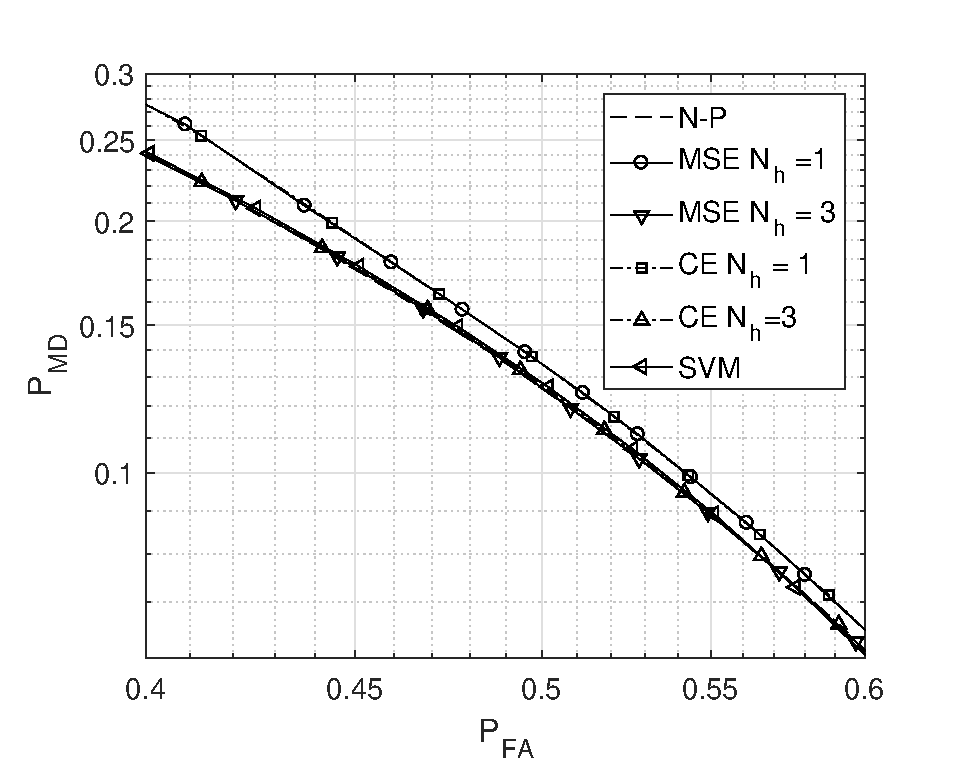
\includegraphics[width=0.6\columnwidth]{res_com_CE_MSE_SVM.eps}
    \caption{\ac{md} probability vs. \ac{fa} probability in the scenario of Section \ref{sec:los}. Comparison between the \ac{np} test function, \ac{svm} and \ac{mlp} with $N_h$ neurons in the hidden layer and both \ac{mse} (NN-\ac{mse} in the legend) and CE training (NN-\ac{ce} in the legend).}
    \label{fig:ceVSmse}
\end{figure}

In this section we present numerical results obtained using the proposed solutions for the scenario described in Section II. In particular, for the \ac{nn} (in two-class classification) the activation function of the input layer is the identity function, while the activation function of the hidden layers is the sigmoid function
\begin{equation}
\psi^{(\ell)}(x) = \frac{1}{1-e^{-x}}.
\end{equation}
The activation function of the output layer is 
\begin{equation}
\psi^{(L-1)}(x)=\tanh^{-1}(x) = \frac{1}{2} \left( \frac{1+x}{1-x} \right).
\end{equation}

We also consider  a unitary transmitting power for each user and a carrier frequency of $2.12$ GHz. The path-loss coefficient is $\nu=3$, the shadowing power is $\sigma_s^2=3.39$ and the shadowing decorrelation distance is $d_c=75$ m. 


\subsection{Two-classes \ac{irlv} With Single \ac{ap}}

We consider here the \ac{irlv} system using a single \ac{ap}. Two channel models are considered: a simple \ac{los} channel model as discussed in Section \ref{sec:los} and a no-\ac{los} model including both path-loss and shadowing.

In order to build the training set we consider $n_x$ spatial points $\bm{x}_{\rm ue}$, each one representing the coordinates of the position of a \ac{ue}, uniformly distributed over the area $\mathcal A$.


\paragraph*{\ac{los} Model} We first consider the simplified scenario of Section \ref{sec:los} in order to have a simple implementation of the \ac{np} test function.  We consider an overall circular area $\mathcal{A}_0$ with radius $40$ m., a squared authentic area $\mathcal{A}_1$ of $625$ m$^2$ located inside $\mathcal{A}_0$, with upper left corner at a distance of $4$ m. from the center of $\mathcal{A}_0$. We considered $10^6$ training points. For the \ac{nn} solution we considered various values for the number $N_h$ of the neurons in the hidden layer.


Fig. \ref{fig:ceVSmse} shows the \ac{fa} versus (vs.) the \ac{md} probabilities -- the so-called \ac{roc} --  obtained with various \ac{irlv} techniques. In particular we compare the \ac{np} detector with \ac{svm} and and \ac{mlp} with $N_h$ neurons in the hidden layer and both \ac{mse} and CE training. 

We first notice that the \ac{ce}-trained and the \ac{mse}-trained \acp{mlp} obtain the same performance when considering the same number of neurons $N_h$. This confirms that the two training methods are performing hypothesis testing in an equivalent manner. Furthermore we notice that as the number of neurons in the hidden layer grows the performance of the \ac{mlp} classifiers approaches that of the optimal \ac{np} classifier, and the equivalence is reached already with $N_h=3$ neurons. This confirms that both \ac{ce}-trained and \ac{mse}-trained \acp{mlp} at convergence are performing the optimal \ac{np} test and that convergence is obtained with a small number of neurons. Furthermore we notice that the \ac{svm} attains the same performance of the \ac{mlp} with $N_h = 3$ and hence of the \ac{np} detector, confirming again that \ac{svm} is optimal in the \ac{np} sense.

In general, the achieved $(P_{\rm FA}, P_{\rm MD})$ probability couples show quite high values: this is due to the fact that a single \ac{ap} is used for \ac{irlv}, and there are many points outside the \ac{roi} that are at the same distance from the \ac{ap} of those inside the \ac{roi}. Since the attenuation is a function only of this distance, there is a huge ambiguity in the attenuation of points inside and outside the \ac{roi}.

\paragraph*{No-LOS Scenario} 

\begin{figure}[t]
    \centering
    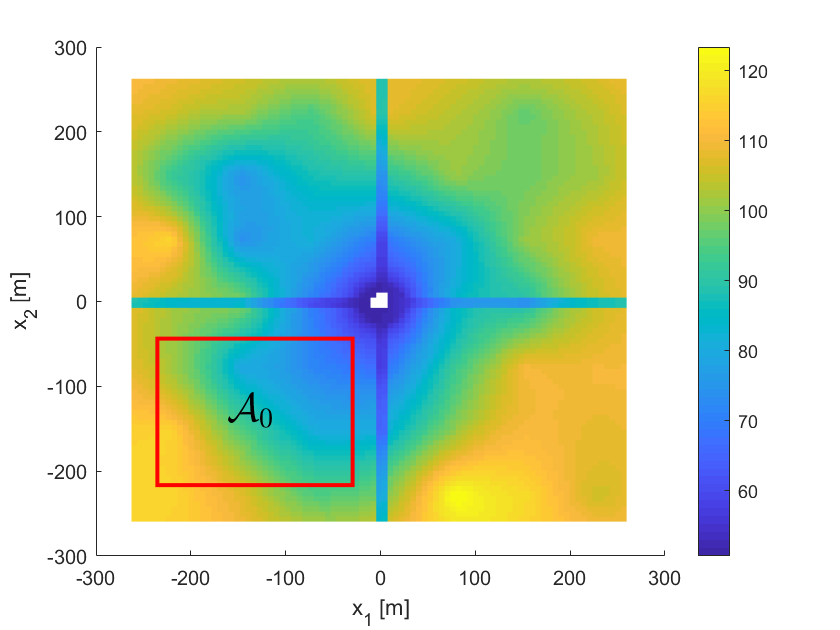
\includegraphics[width=0.6\columnwidth]{surfColorato.png}
    \caption{Example of attenuation map including path-loss and shadowing in the non-\ac{los} scenario.}
    \label{fig:map}
\end{figure}

We now consider a more general scenario including shadowing and no-\ac{los}. In particular, we consider a Manhattan grid with two streets crossing at the center of a square region. Along the the streets \ac{los} propagation conditions are present, while no-\ac{los} propagation conditions are present in the rest of the area. Fig. \ref{fig:map} shows a realization of the  attenuation map including path-loss and shadowing when the \ac{ap} is located at the map center. In the figure we have also indicated the \ac{roi} $\mathcal{A}_0$. Furthermore we note the \ac{los} attenuations along the streets.

Again, using a single \ac{ap} we do not expect to be able to achieve low \ac{md} and \ac{fa} probability. Indeed, when compared to the \ac{los} scenario the presence of shadowing increases the ambiguity on the attenuation inside and outside the region. However in this simple scenario we can drive some relevant results in the comparison of the considered \ac{irlv} techniques. 


%Consider the \ac{llr} (\ref{eq:lr}). In the no-\ac{los} context the computation of the two area dependent probabilities has no closed-form solution. A numerical solution is obtained by sampling the attenuation values over the spatial grid of positions and computing the area dependent distributions of the attenuation values. Consider an attenuation value $\hat{a}$: the probability of measuring $\hat{a}$ given that the \ac{ue} is located in area $\mathcal{A}_0$ is given by the number of positions $(x_u,y_u) \in \mathcal{A}_0$ where the measured attenuation $a(x_u,y_u)=\hat{a}$ over the total number of positions $(x_u,y_u)$ in the entire map having the same attenuation $\hat{a}$, i.e.
%\begin{equation}
%    \mathbb{P}(\hat{a}|\mathcal{A}_0) \approx \frac{\text{number of positions} \, (x_u,y_u) \in \mathcal{A}_0 \, \text{s.t.} \, a(x_u,y_u) = \hat{a}}{\text{total number of positions} \, (x_u,y_u) \, \text{s.t.} \, a(x_u,y_u) = \hat{a}}
%\end{equation}
%With the same reasoning we compute $\mathbb{P}(\hat{a}|\mathcal{A}_1)$, and an approximation of equation (\ref{eq:lr} is hence obtained as
%\begin{equation}\label{eq:lrApp}
%    \mathcal{L} \approx \frac{\text{number of positions} \, (x_u,y_u) \in \mathcal{A}_0 \, \text{s.t.} \, a(x_u,y_u) = \hat{a}}{\text{number of positions} \, (x_u,y_u) \in \mathcal{A}_1 \, \text{s.t.} \, a(x_u,y_u) = \hat{a}}
%\end{equation}
%The value computed by (\ref{eq:lrApp}) gets closer to the real value as the number of grid points over the map increases, as an higher number of points means a better statistical characterization of the attenuation over the map area.

The first question we address is if we can implement the \ac{np} approach when the channel model is more complicated or not known a-priori. In this case we could quantize the attenuation values with a large alphabet and estimate the sampled \ac{pdf} for the quantized attenuation using a large number of training point. For the considered scenario with path-loss and shadowing we use $4.46 \cdot 10^6$ training points in the area and a uniform quantizer for the attenuation was considered with $300$ quantization values. Fig. \ref{fig:trueMap} shows the \ac{md} probability vs. the \ac{fa} probability obtained for the attenuation map of Fig. \ref{fig:map}. In particular we here compare the results obtained by (\ref{eq:lrApp}) with the results obtained with \ac{ml}-based approaches. \Ac{mlp} si trained with \ac{mse} loss function and results are shown for different number of neurons $N_h$ in the hidden layer.

For training of both \ac{mlp} and \ac{svm} we used $10^3$ points. We notice that both the \ac{mlp} and the \ac{svm} outperform the \ac{np}-based detector. This means that even if we considered a much larger number of training points for the estimation of the \ac{pdf} to be used in the \ac{llr} computation, still we have a performance degradation with respect to the optimal approach. On the other hand a smaller number of training points provide a more powerful test function by using \ac{ml} approaches. Therefore in the following we drop the \ac{np} method and we consider long training and many neurons for the \ac{ml} in order to achieve close-to-optimal performance.

Still from Fig. \ref{fig:trueMap} we see that with $N_h=10$ the \ac{mlp} and the \ac{svm} attain the same performance. 

\begin{figure}[t]
    \centering
    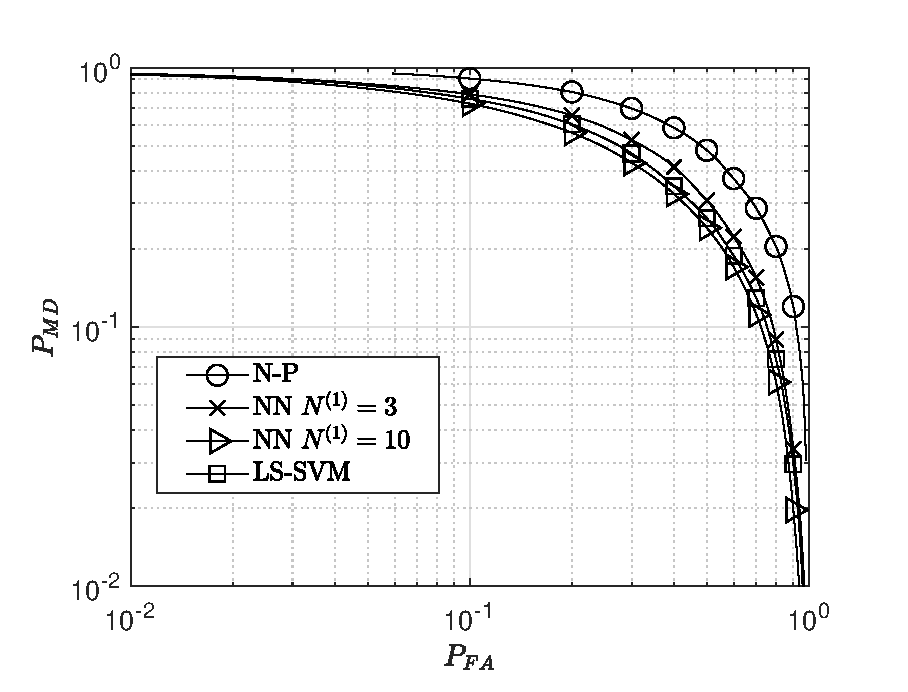
\includegraphics[width=0.6\columnwidth]{res_NP_approx_SVM.eps}
    \caption{\ac{md} probability vs \ac{fa} probability for the attenuation map in Fig. \ref{fig:map} for \ac{np}, \ac{svm} and \ac{nn} with MSE design and with $N_h$ neurons in the hidden layer.}
    \label{fig:trueMap}
\end{figure}

%Comparing the number of grid points and the number of training points used for the \ac{ml} algorithms we can conclude that the \ac{ml}-based solution is advantageous over the \ac{np}-based one, as it requires a smaller number of points in order to get an estimate of the area dependent probabilities. Furthermore this implies that the \ac{ml}-based \ac{irlv} system can be implemented without any a-priory knowledge of the \ac{pdf} of the hypothesis to be tested.

\subsection{Two-classes \ac{irlv} With Multiple \acp{ap}}\label{sec:res_fading}

We now consider the network of Fig. \ref{fig:mBS}, with $N_{\rm ap}=5$ \acp{ap} collecting attenuation values of their channels to the \acp{ue}. As already mentioned, due to the difficulty of obtaining the performance of \ac{np} we focus here on \ac{ml} in an asymptotic regime of training points and complexity. Moreover, thanks to the presence of multiple \acp{ap}, we can better distinguish attenuations vectors associated to \ac{ue} positions inside and outside the \ac{roi}. Lastly, we now include also fading into the channel model, as discussed in Section II.

\begin{figure}[t]
    \centering
    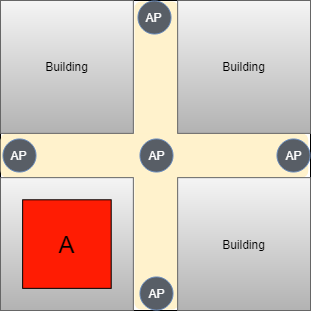
\includegraphics[width=0.5\columnwidth]{scenario2.png}
    \caption{Scenario with 5 \acp{ap}.} 
    \label{fig:mBS}
\end{figure}
\begin{figure}[t]
    \centering
    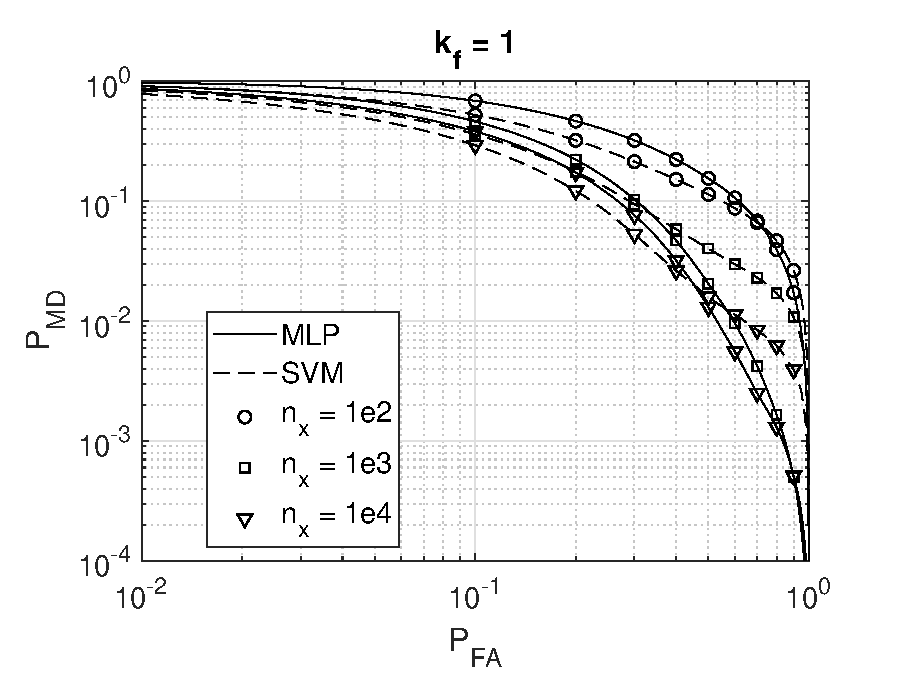
\includegraphics[width=0.6\columnwidth]{res_avg_nTrain_kf1.eps}
    \caption{$P_{\rm MD}$ vs. $P_{\rm FA}$ for different number of space points $n_x$ and one ($k_f=1$) fading realization per space point. The NN-based \ac{irlv} is implemented with $N_h = 10$ and \ac{ce} loss function.}
    \label{fig:kf1}
\end{figure}

\begin{figure}[t]
    \centering
    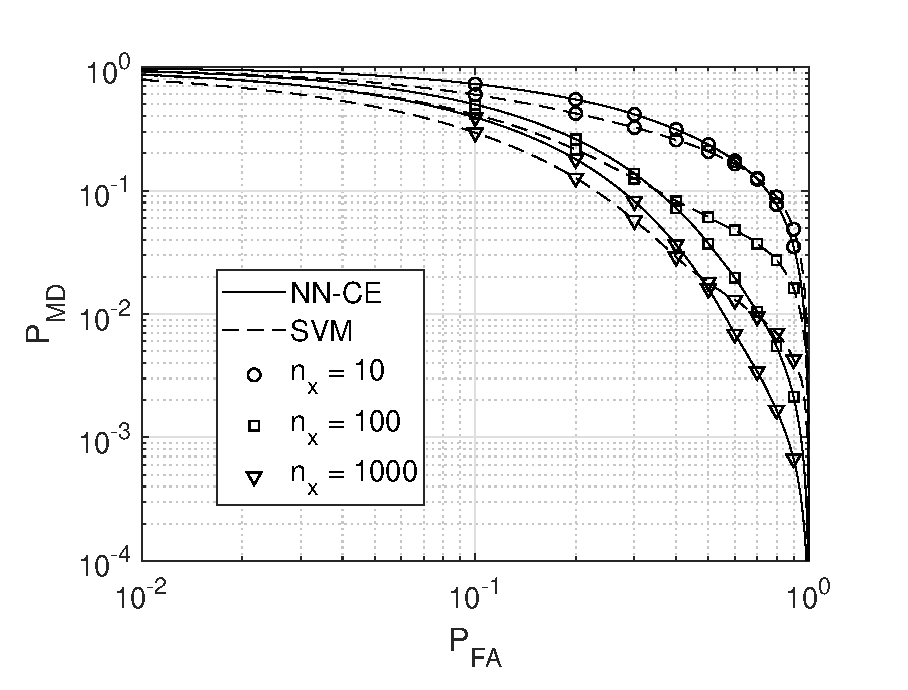
\includegraphics[width=0.6\columnwidth]{res_avg_nTrain_kf10.eps}
    \caption{\ac{md} vs. \ac{fa} probabilities for different numbers $n_x$ of space points and $k_f=10$ fading realizations per space point. The NN-based \ac{irlv} is implemented with $N_h = 10$ and \ac{ce} loss function.}
    \label{fig:kf10}
\end{figure}

Consider a realization of the shadowing map as depicted in Fig. \ref{fig:map}. A single position $\bm{x}_{\rm ue}$ is associated to a single shadowing value, however since we also include fading effects, the attenuation vectors measured by the \acp{ap} are different in different time instants even for the same \ac{ue} position $\bm{x}_{\rm ue}$. We then aim at establishing the performance of the \ac{irlv} techniques according the number of different fading realization that are collected in the learning phase for each point in space. Let $n_x$ be the number of spatial points explored by the \ac{ue}, whereas for each point we collect $k_f$ fading realizations, for a total of $S = n_x \cdot k_f$ training attenuation vectors. 

Fig.s \ref{fig:kf1} and \ref{fig:kf10} show the \ac{roc} of various \ac{irlv} techniques for different values of collected space points $n_x$ and number of fading realization $k_f = 1$ and $10$ per space point. Results are reported in solid line for the \ac{mlp} and in dashed line for the \ac{svm} . The \ac{mlp} has been implemented with $N_h=10$ and \ac{ce} loss function.  Comparing the two figures we note that, for a given training set value $S$, performance get worse as the number of fading realization grows. However we also notice that, for a given number of spatial position $n_x$, performance are better if we consider a larger number of fading realizations. Furthermore we see that, for a large enough training set,  different values $k_f$ provide approximately the same performance.  Therefore we can conlude that, for large training sets \ac{ml} algorithms are also robust to fading. 


\subsection{One-Class \ac{irlv} With Multiple \acp{ap}}


We consider here the one-class \ac{irlv} solutions, where the training points come only from the \ac{roi} $\mathcal A_0$. Note that the performance of the  \ac{ae}-based \ac{irlv} depends on its compressing capability and hence on the number of neurons $N_h$ in the hidden layer.  

We first consider a scenario with path-loss and shadowing only, thus without fading. Fig. \ref{fig:aeNh} shows the \ac{roc} for the one class \ac{irlv} for both \ac{oclssvm} and \ac{ae} with $N_h \in [1, 5]$. $S=10^4$ training vectors have been used for training and only path loss and shadowing effects are considered. We see that by increasing $N_h$ the performance of \ac{ae}-based \ac{irlv} does not improve: indeed, the optimum \ac{roc} is obtained for $N_h=2$. This is due to the fact that  \ac{ae} compresses the attenuation vectors and hence best performance are achieved when it  extracts the optimal number of features from the input. Furthermore we notice that the \ac{oclssvm} is a more effective classifier than the \ac{ae}, as the obtained \ac{roc} attains lower $P_{\rm MD}$ values for the same $P_{\rm FA}$ values.

\begin{figure}[t]
    \centering
    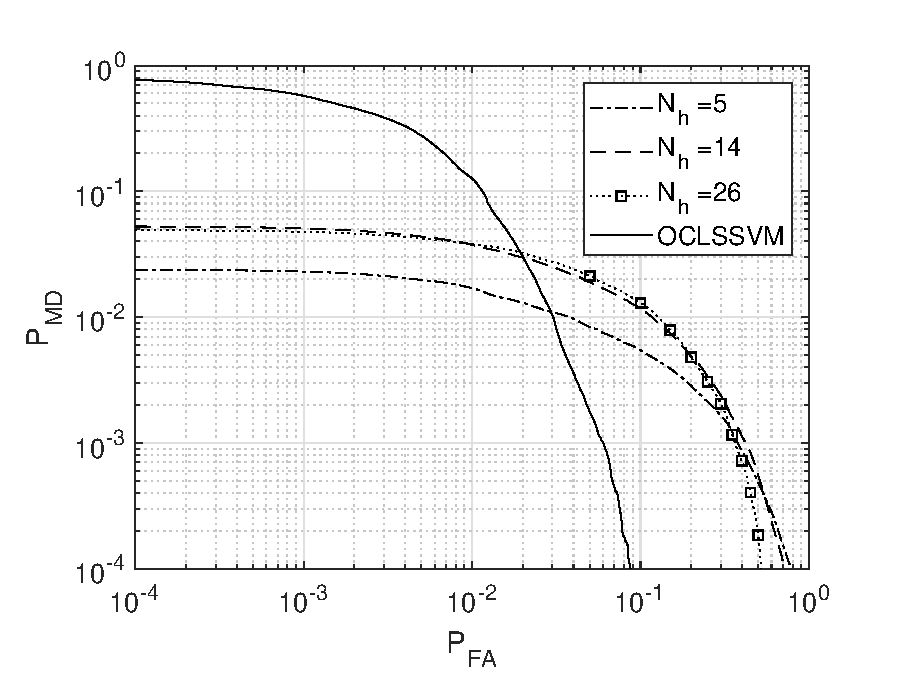
\includegraphics[width=0.6\columnwidth]{res_ae_onNeur.eps}
    \caption{\ac{md} vs. \ac{fa} probability of one-class \acp{irlv} in a scenario with path-loss, shadowing and without fading. \ac{ae} performance are shown for different values of $N_h$.}
    \label{fig:aeNh}
\end{figure}
 
We now consider the effect of the training set size $S$. Note that for one-class \ac{irlv} the training set collects only attenuation vectors from \ac{ue} located in $\mathcal{A}_0$, whereas the testing set comprises attenuation vectors of \acp{ue} both inside and outside $\mathcal A_0$. As in Section \ref{sec:res_fading} we consider a training set with size $S = n_x \cdot k_f$ and we test and compare the training sets created with $k_f=1$ and $10$.

Fig.s \ref{fig:kf1Oc} and \ref{fig:kf10Oc} show $P_{\rm MD}$ vs. $P_{\rm FA}$ of \ac{irlv} systems based on  both \ac{ae} and \ac{oclssvm}, for $k_f = 1$ and $10$.  Results are reported in solid line for the \ac{ae} and in dashed line for the \ac{oclssvm}. The \ac{ae} has been implemented with $N_h=2$. Different markers denote various training set size values $k_t$.

We first notice that the \ac{ae} is less sensitive to the training set size, as different values of $k_t$ attain approximately the same performance both for $k_f=1$ and $10$. Furthermore we note that for $P_{\rm FA} > 10^{-1}$ the \ac{oclssvm} attains a lower  $P_{\rm MD}$. Moreover, we note that the \ac{ae}-\ac{irlv} is not sensitive to noise, as error probabilities are very similar in both figures. Instead we notice that  \ac{oclssvm} is more sensitive to noise for small set sizes. In fact we notice that for $S=10^2$ performance is different for $k_f=1$ and $10$. Instead, as $S$ grows, performance is almost the same for both values of $k_f$. Furthermore we notice that for small $S$ it is better to use one fading realization per space point ($k_k=1$) in building the training set for the \ac{oclssvm}. This is different  from what we observed for two-class classification, where taking more fading measures provided an advantage.  

Comparing one-class and two-class classification in Fig.s \ref{fig:kf1} and \ref{fig:kf10} we note that  one-class \ac{svm}-\ac{irlv} outperforms  two-class solutions for large training sets and  both values of $k_f$ and $P_{\rm FA}>10^{-1}$. When considering the \ac{nn}-based algorithms we see that one-class classification outperforms the two-class solution for small training set sizes, while the performance are swapped for large $S$ values and $P_{\rm FA} > 10^{-1}$. This result holds for both values of $k_f$. Furthermore we see that \ac{oclssvm} outperforms \ac{mlp} when considering the same values of $n_x$ and $S$ and $P_{\rm FA}> 10^{-1}$.


\begin{figure}[t]
    \centering
    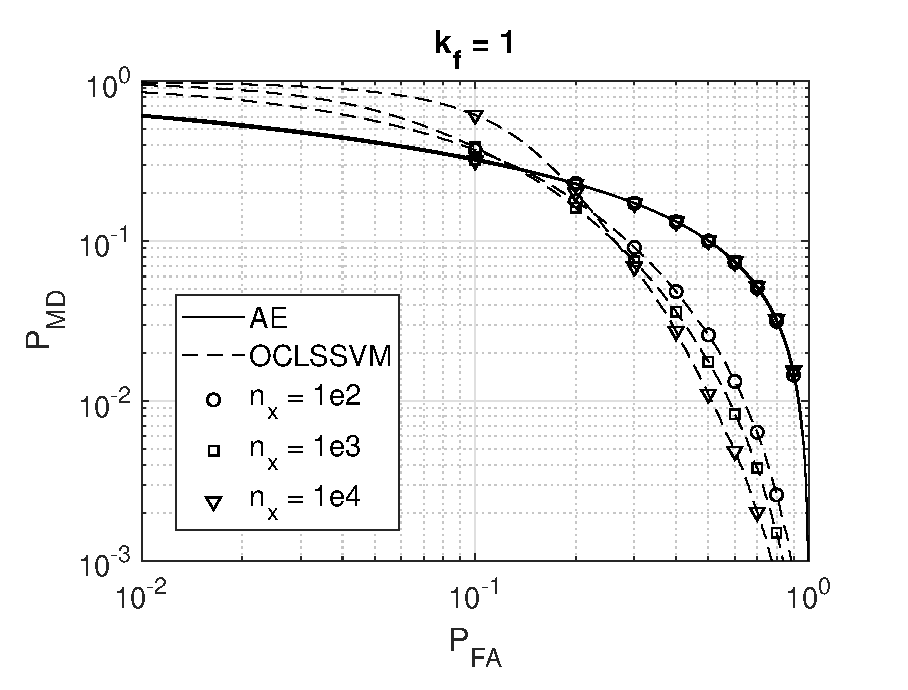
\includegraphics[width=0.6\columnwidth]{res_avgnTrain_oneClass_kf1.eps}
    \caption{\ac{roc} for one-class \acp{irlv} in a scenario with path-loss, shadowing and fading with different training set size and $k_f=10$ fading realizations,  \ac{ae} with $N_h = 2$. }
    \label{fig:kf1Oc}
\end{figure}

\begin{figure}[t]
    \centering
    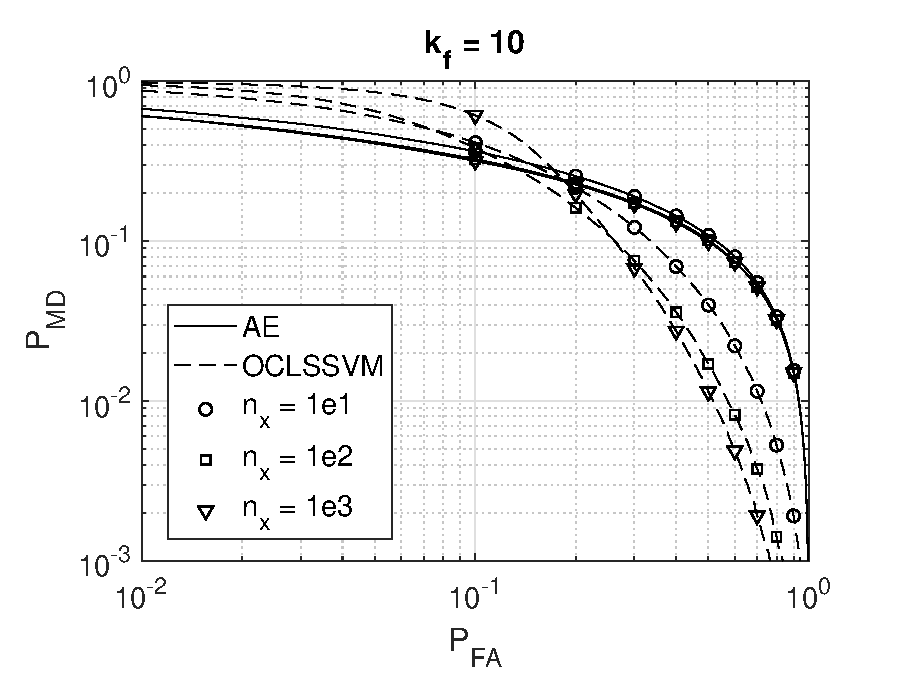
\includegraphics[width=0.6\columnwidth]{res_avgnTrain_oneClass_kf10.eps}
    \caption{Convergence of the \ac{ae}. $P_{\rm MD}$ vs. $P_{\rm FA}$ for \ac{ae} with $N_h = 2$, different training set size and $k_f=10$ fading realizations.}
    \label{fig:kf10Oc}
\end{figure}

\subsection{\ac{ml} Attack Strategies}

We consider now the \ac{ml} attack strategies described in Section \ref{sec:attack} for the scenario of Fig. \ref{fig:mBS} and channels including path loss, shadowing and fading. The \ac{irlv} is also implemented with one-class classifiers. 

%In order to test the attacks we set the \ac{fa} probability at the defense side, such that the threshold value needed for classification is given. We compare attacks and defense both implemented via \ac{ae} and \ac{oclssvm}. 

We compare the \ac{ml} attack strategies with uniformly random attacks, wherein attacks are launched by uniformly random positions in the \ac{roi}-complementary area $\mathcal{A}_1$.  Moreover, as a naive enhancement we consider a \emph{random-border} attack, wherein the attacker moves only along the border between areas $\mathcal{A}_0$ and $\mathcal A_1$, as we expect that being closer to the \ac{roi} increases the chances of a successful attack. The same \ac{ml} algorithm is implemented for one-class classification at both attack and defense sides, although the attacker training is with points in $\mathcal A_1$, while the \ac{ap} network training is with points in $\mathcal A_0$. For the \ac{irlv} training we set $k_f=10$.

Fig.s \ref{fig:selectiveSVM} and \ref{fig:selectiveAE} show the \ac{cdf} of the time of first successful attack $\eta$ for three attack strategies, namely the random, random-border and selective ML strategies. Fig. \ref{fig:selectiveAE} shows results when both attack strategies and \ac{irlv} are based on \acp{ae}, with $P_{\rm FA} =0.5$ for the network. We observe that the random-border attack outperforms the pure random attack, while still being less-powerful than selective \ac{ml}. Similarly, Fig. \ref{fig:selectiveSVM} shows the \ac{cdf} of $\eta$ for \ac{irlv} with $P_{\rm FA}=10^{-2}$ and both the attack strategies and the \ac{irlv} based on \ac{oclssvm}. In this case selective-ML attack outperforms the pure random attack, while the two random attacks perform closely. We can conclude that the \ac{ml} selective attack is clearly reducing the time to reach a success with respect to random attacks. Moreover, \ac{oclssvm} is more robust to attacks than \ac{ae} when used for \ac{irlv}, as the \ac{fa} probability for \ac{irlv} is much smaller than that achieved by \ac{ae}.



\begin{figure}[t]
    \centering
    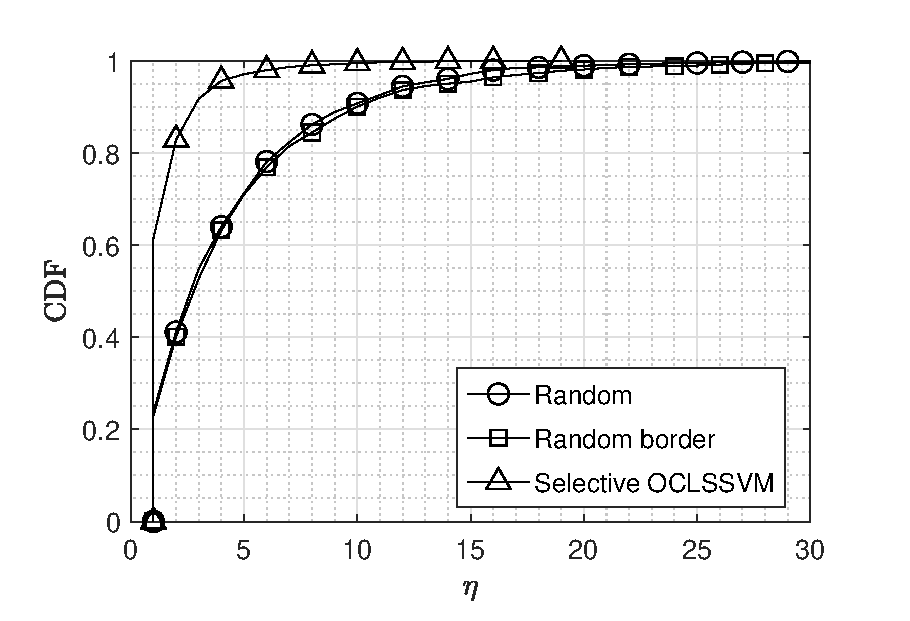
\includegraphics[width=0.6\columnwidth]{res_selective_SVM.eps}
    \caption{Convergence of the \ac{ae}. $P_{\rm MD}$ vs. $P_{\rm FA}$ for \ac{ae} with $N_h = 2$, different training set sizes and $k_f=10$ fading realizations.}
    \label{fig:selectiveSVM}
\end{figure}

\begin{figure}[t]
    \centering
    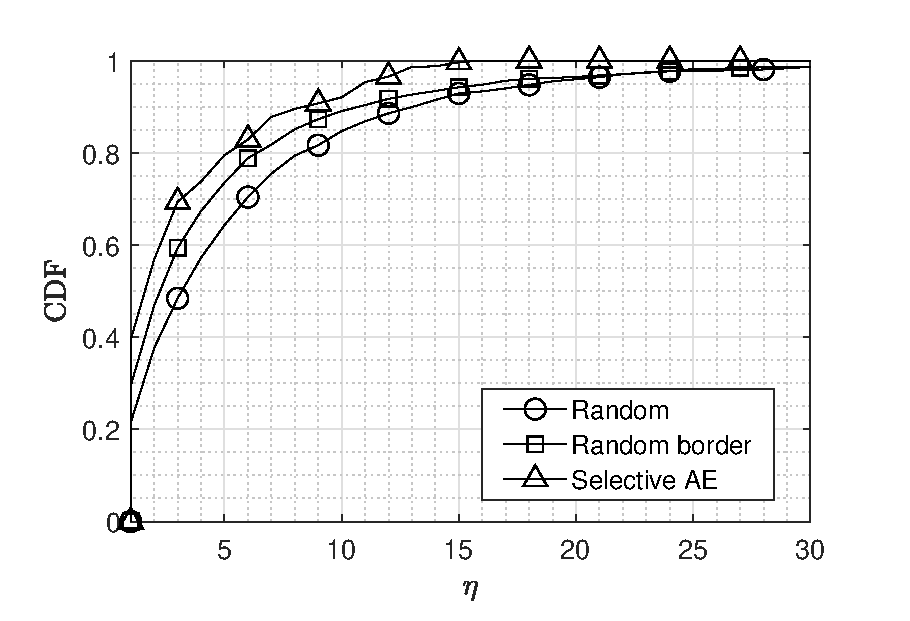
\includegraphics[width=0.6\columnwidth]{res_selective_AE.eps}
    \caption{Convergence of the \ac{ae}. $P_{\rm MD}$ vs. $P_{\rm FA}$ for \ac{ae} with $N_h = 2$, different training set sizes and $k_f=10$ fading realizations.}
    \label{fig:selectiveAE}
\end{figure}

\section{Conclusions}

In this paper we have proposed innovative solutions for the \ac{irlv} in wireless networks that exploit the  features of the channels between the \ac{ue} whose location must be verified and a trusted network of \acp{ap}. From the observation that in practical situations the statistics of the channel is not available to the network infrastructure, we proposed \ac{ml}-based solutions, operating with both one- and two-class classification, i.e., with assumptions on attack statistics or not. For two-class classification we have proved that  both \ac{nn} and \ac{svm} solutions based on various design criteria are most powerful tests for a given sensitivity, i.e., they are equivalent to the \ac{np} test. Instead, one-class classification both \ac{ae} and \ac{svm} solutions are not equivalent to the \ac{glrt}. From numerical results we conclude that \ac{ml} converges to optimal performance with much smaller training set sizes than direct estimation of \ac{np} test. We have also investigated the impact of various wireless propagation phenomena investigating how to collects points for training in order to be robust against these phenomena.

\section*{Appendix}

	Given a finite  attenuation vector alphabet $\mathcal C = \{\bm{\alpha}_1, \ldots, \bm{\alpha}_M\}$ of $M$ elements, with $\bm{a}^{(i)} \in \mathcal C$, we indicate with $p_{\bm{a}^{(i)},t_i}(\bm{\alpha}_j, t)$, with $t \in \{-1,1\}$, the joint probability of input vector $\bm{a}^{(i)}$ and corresponding output $t_i$, $i=1, \ldots, S$.
	
	By the Glivenko–Cantelli theorem we have that with probability 1 as $S\rightarrow \infty$ there are $Sp_{\bm{a}^{(i)},t_i}(\bm{\alpha}_j,t)$ training vectors $\bm{\alpha}_j$ with associated true value $t$ in any training sequence.
	All these training points will have the same value $e_i$, from (\ref{eq:stpart}), that will appear $Sp_{\bm{a}^{(i)},y_i}(\bm{\alpha}_j,t)$ times in the sum $\sum_{i=1}^{S} e_i^2$.
	Note that in the training ensemble there could be two equal instances $\bm{a}^{(m)}=\bm{a}^{(n)}=\bm{\alpha}_j$, but with different labels $t_m \neq t_n$. Therefore, for $\bm{a}^{i}=\bm{\alpha}_j$ we can have two possible values for $e_i$, depending on $y_i$, and we denote them with $e_{j,1}$ and $e_{j,-1}$.
	This translates in only $2M$ \textit{distinct} constraints of the type \eqref{eq:stpart}.
	Asymptotically, for $S \to \infty$, problem (\ref{eq:lssvm}) becomes
	\begin{subequations}
		\label{eq:lssvm22}
		\begin{equation}
		\label{eq:lssvm2}
		\underset{\bm{w},e}{\text{min}} \quad f_l' \triangleq \frac{1}{2} \bm{w}^T \bm{w} + C S \frac{1}{2} \sum_{j=1}^M [p_{\bm{a}^{(i)},t_i}(\bm{\alpha}_j,1) e_{j,1}^2 + p_{\bm{a}^{(i)},y_i}(\bm{\alpha}_j,-1) e_{j,-1}^2]  
		\end{equation}
		subject to 
		\begin{equation}
		\label{eq:stpart2}
		[\bm{w}^T \phi (\bm{\alpha}_j) + b] = 1- e_{j,1}\quad j = 1 ,\dots,M.
		\end{equation}
		\begin{equation}
		\label{eq:stpart3}
		\quad  -[\bm{w}^T \phi (\bm{\alpha}_j) + b] = 1- e_{j,-1}\quad j = 1 ,\dots,M.
		\end{equation}
	\end{subequations}
	whose solution provides the convergence value (in probability) of vector $\bm{w}$. We write the Lagrangian
	\begin{equation}
	\mathcal{L}_1 = f_l' - \sum_{k=1}^{M} v_k \left[ \bm{w}^T \phi (\bm{\alpha}_j) + b - 1 + e_{j,1} \right] 
	- \sum_{k=1}^{M} u_k \left[- \bm{w}^T  \phi (\bm{\alpha}_j) - b  - 1 + e_{j,-1} \right], 
	\end{equation}
	where $\{u_k,v_k\}_{k=1}^{M}$ are the Lagrangian multipliers. Let us set to zero the derivatives w.r.t. $\{\bm{w},b,e_{j,1},e_{j,-1}, v_j,u_j\}$
	\begin{subequations}
		\begin{equation}
		\label{eq:deriv1_1}
		\frac{\partial \mathcal{L}_1}{ \partial \bm{w}}: \quad \bm{w} = \sum_{k=1}^{M} (u_k - v_k) \phi (\bm{\alpha}_k),
		\end{equation}
		\begin{equation}
		\label{eq:deriv1_2}
		\frac{\partial \mathcal{L}_1}{\partial b}: \quad \sum_{k=1}^{M} (u_k - v_k) = 0 ,
		\end{equation}
		\begin{equation}
		\label{eq:deriv1_3}
		\frac{\partial \mathcal{L}_1}{\partial e_{j,1}}: \quad v_j = CSp_{\bm{a}^{(i)},t_i}(\bm{\alpha}_j,1) e_{j,1} \quad j=1\dots M,
		\end{equation}
		\begin{equation}
		\label{eq:deriv1_4}
		\frac{\partial \mathcal{L}_1}{\partial e_{j,-1}}: \quad u_j = CSp_{\bm{a}^{(i)},t_i}(\bm{\alpha}_j,-1) e_{j,-1} \quad j=1\dots M,
		\end{equation}
		\begin{equation}
		\label{eq:deriv1_5}
		\frac{\partial \mathcal{L}_1}{\partial v_j}: \quad \bm{w}^T \phi (\bm{\alpha}_j) + b - 1 + e_{j,1} = 0 \quad j=1\dots M,
		\end{equation}
		\begin{equation}
		\label{eq:deriv1_6}
		\frac{\partial \mathcal{L}_1}{\partial u_j}: \quad - \bm{w}^T \phi (\bm{\alpha}_j) - b - 1 + e_{j,-1} = 0 \quad j=1\dots M.
		\end{equation}
	\end{subequations}
	Substituting \eqref{eq:deriv1_1}, \eqref{eq:deriv1_3} and \eqref{eq:deriv1_4} in \eqref{eq:deriv1_5} and \eqref{eq:deriv1_6} we get the system of equations
	\begin{subequations}
		\label{eq:system1}
		\begin{equation}
		\sum_{k=1}^{M} (u_k - v_k) k(\phi (\bm{\alpha}_k,\bm{\alpha}_j)) + b - 1 + \frac{v_j}{CSp_{\bm{a}^{(i)},t_i}(\bm{\alpha}_j,1)} = 0
		\quad j=1\dots M
		\end{equation}
		\begin{equation}
		- \sum_{k=1}^{M} (u_k - v_k) k(\phi (\bm{\alpha}_k,\bm{\alpha}_j)) - b - 1 + \frac{v_j}{CSp_{\bm{a}^{(i)},t_i}(\bm{\alpha}_j,-1)} = 0
		\quad j=1,\dots, M
		\end{equation}
		\begin{equation}
		\sum_{k=1}^{M} (u_k - v_k) = 0.
		\end{equation}
	\end{subequations}
	\eqref{eq:system1} is a system with $2M + 1$ equations, linear in the $2M + 1$ unknowns $\{u_k,v_k,b\}_{k=1}^{k=M}$ and therefore has finite solution. In particular, using \eqref{eq:deriv1_1}, we have
	\begin{equation}
	\label{eq:wSolution}
	\bm{w}^T\bm{w} =  \sum_{k=1}^{M} \sum_{h=1}^{M} k(\bm{\alpha}_k,\bm{\alpha}_h) (v_kv_h + u_ku_h -2 v_ku_h),
	\end{equation}
	where we used the fact that the kernel function
	\begin{equation}
	k(\bm{\alpha}_k,\bm{\alpha}_h) \triangleq \phi(\bm{\alpha}_k) \phi(\bm{\alpha}_h)^T
	\end{equation}
	 is symmetric \wrt its inputs. 
	
%	Note that while the original problem \eqref{eq:lssvm}, as $S \to \infty$, has infinite constraints, the equivalent formulation \eqref{eq:lssvm22} includes a finite number $2M$ of constraints.
	
	We conclude that $\bm{w}$ has a finite norm since the right hand side of \eqref{eq:wSolution} is a finite sum.
	  


%\bibliographystyle{IEEEtran}
%\bibliography{bibliography.bib}
\renewcommand*{\bibfont}{\footnotesize}

\printbibliography

\end{document}
